\documentclass{book}

\usepackage{bm}
\usepackage{float}
\usepackage{amsmath}
\usepackage{amsfonts}
\usepackage{graphicx}
\usepackage{lineno}
\usepackage{natbib}
\usepackage{hyperref}
\usepackage{verbatim}
\usepackage{soul}
\usepackage{color}

\bibliographystyle{asa}

\floatstyle{plain}
\floatname{panel}{Panel}
\newfloat{algorithm}{h}{txt}[chapter]
\newfloat{panel}{h}{txt}[chapter]


\newcommand{\R}{\textbf{R}}
\newcommand{\bugs}{\textbf{BUGS}}
\newcommand{\jags}{\textbf{JAGS}}
\newcommand{\secr}{\mbox{\tt secr}}
\newcommand{\scrbook}{\mbox{\tt scrbook}}


\linenumbers

\begin{document}


\chapter{Introduction}
\label{chapt.intro}

\chapter{GLMS and WinBUGS}
\label{chapt.glms}

\chapter{Closed population models}
\label{chapt.closed}

\chapter{Fully Spatial capture-recapture models}
\label{chapt.scr0}

\chapter{Other observation models}
\label{chapt.poisson}

\chapter{MLE chapter}
\label{chapt.mle}


\chapter{MCMC chapter}
\label{chapt.mcmc}

\chapter{Goodness of Fit and stuff}
\label{chapt.gof}

\chapter{Covariate models}
\label{chapt.covariates}

\chapter{
Integrating Resource Selection with
Spatial Capture-Recapture
  Models}

\markboth{Resource Selection and Space Usage}{}
\label{chapt.rsf}


\vspace{.3in}

Up to this point we have developed many variations of SCR models to
describe the observation process.  These included models of the
relationship between encounter probability and distance, and different
types of covariates such as behavioral responses that can affect
detection probability.  Although these different observation models
are immensely useful, they are rather basic in the sense that they
imply simplistic models of how individuals use space (section
\ref{scr0.sec.implied}) and how individuals are distributed in space.
In the following several chapters we generalize some of the core SCR
assumptions to accommodate more realistic notions of how animals use
space.  


In Sec. \ref{scr0.sec.implied}
we briefly discussed the notion of how SCR encounter probability
models relate to models of space usage.
When we use symmetric and
stationary encounter probability models, SCR models 
imply that space usage is a decreasing function of distance from an
individuals home range center.  In this chapter,
we extend SCR models to incorporate models of resource selection (RS),
such as when one or more explicit landscape covariates are available
which the investigator believes might affect how individual animals
use space within their home range (this is what \citep{johnson:1980}
called {\it third-order} selection).  Our treatment follows
\citet{royle_etal:2012mee} who integrated a standard family of
resource selection models based on auxilliary telemetry data into the
capture-recapture model for encounter probability.  The approach is
consistent with the manner in which classical ``resource selection
function'' (RSF) models \citep{manly_etal:2002} or utilization
distributions \citep{worton:1989, fieberg:2005, fieberg:2007} are
estimated from animal telemetry data.  \citet{royle_etal:2012mee}
argued that SCR models and resource selection models estimated from
telemetry are based on the same basic underlying model of space
usage. The important distinction between SCR and RSF studies are that,
in SCR studies, encounter of individuals is imperfect (i.e.,
``$p<1$'') whereas, with RSF data obtained by telemetry, encounter is
perfect (or, rather, detection is not a {\it stochastic} outcome). We
can think of the two as being exactly equivalent either if we have a
dense array of trapping devices, or if our telemetry apparatus is
imperfect such as only samples a small area of space (this would be
consistent with telemetry stations for sampling fish which only
measure passage).



Telemetry studies are extremely common in animal ecology for studying
movement and resource selection, and SCR studies frequently obtain
such data on a subset of individuals. Thus, formal integration of
capture-recapture with telemetry data for the purposes of modeling
resource selection has a number of immediate benefits. For one, 
 telemetry data provide direct information about $\sigma$
\citep{sollmann_etal:2012ecol,sollmann_etal:inprepjapplecol}. As a
result, this leads to improved estimates of model parameters, and also
has design consequences (see Sec. \ref{design.sec.telemetry}).  In
addition, active resource selection by animals induces a type of heterogeneity in
encounter probability, which is misspecified by standard SCR encounter
probability models. As a result, estimates of population size or
density under models that do not account for resource selection can be
biased \citep{royle_etal:2012mee}.  Finally, because the resource
selection model translates directly to a model for encounter
probability for spatial capture-recapture data, the implication of
this is that it allows us to estimate resource selection model
parameters directly from SCR data, i.e., {\it absent} telemetry
data. This fact should broaden the practical relevance of spatial
capture-recapture for studying or estimating not just density, but
also for directly studyin movement and resource selection.

Telemetry data has been widely 
used in conjuncation with capture-recapture data.  For
example, \citet{white_shenk:2001} and \citet{ivan:2012} suggested
using telemetry data to estimate the probability that an
individual is exposed to sampling. However, their estimator requires that
individuals are sampled in proportion to this unknown quantitiy, which
seems impossible to acheive in many studies. In addition, they do not
directly integrate the telemetry data with the capture-recapture model
so that common parameters are jointly estimated.
\citet{sollmann_etal:inprepjapplecol} and
\citet{sollmann_etal:2012ecol} used telemetry data to directly inform
the parameter $\sigma$ from the bivariate normal SCR model in order to
improve estimates of density, although these models did not include an
explicit resource selection component.



%%% one idea is to use these models to account for sampling along
%%% trails.
%%% define z(x) = trail density or average distance to trail




\section{A Simple Model of Space Usage}
\label{rsf.sec.rsfmodel}

We assume here that our landscape is defined in terms of a discrete
raster of one or more covariates, having the same dimensions and
extent.  Let ${\bf x}_{1},\ldots,{\bf x}_{nG}$ identify the center
coordinates of $nG$ pixels that define a landscape.  We organize these
coordinates into the matrix ${\bf X}_{nG \times 2}$.  Let $z({\bf x})$
denote a covariate measured (or defined) for every pixel ${\bf
  x}$. For clarity, and without loss of generality, we develop the
basic ideas here in terms of a single covariate.  We suppose that a
population of individuals wanders around space in some manner related
to the covariate $z({\bf x})$, and their locations accumulate in
pixels by some omnipotent accounting mechanism. We will define ``use
of ${\bf x}$'' to be the event that an individual animal appeared in
some pixel ${\bf x}$ during some interval of time.

 As a biological matter,
use is the outcome of individuals moving around their home range \citep{hooten_etal:2010},
i.e., where an individual is at any point in time is the result of
some movement process. However, to understand space usage, it is not
necessary to entertain explicit models of movement, just to observe
the outcomes, and so we don't elaborate further on what could be
sensible or useful models of movement, but we imagine existing methods
of hierarchical or state-space
models are suitable for this purpose \citep{jonsen_etal:2005,
  forester_etal:2007, patterson_etal:2008, hooten_etal:2010,
  mcclintock_etal:2012}.
XXX Also cite Ovasakinen papers XXXXXX
We consider explicit movement models in the context of SCR models
later chapters of this book
(Chapt. XXX and XXXX).


If an individual moves from a pixel x to another pixel x' this is
defined as a decision to ``use'' pixel x'. This also induces a
definition of ``truth'' -- that is, over any prescribed time
interval, the animals makes some number, say $R$ of use decisions, and
they are, conceivably, observable by our omnipotent accounting
mechanism (e.g., continuous telemetry).
In this case, 
let $r_{ij}$ be the {\it true} use frequency of pixel $j$ by individual $i$ --
i.e.,
the number of times individual $i$ used pixel $j$.
We assume the 
vector of use frequencies ${\bf r}_{i} = (r_{i1},\ldots,r_{iG})$ has a
multinomial distribution:
\[
{\bf r}_{i} \sim \mbox{Multinom}(R, {\bm \pi}_{i})
\]
where
\[
 \pi_{ij} = \frac{ \exp( \alpha_{2} z({\bf x}_{j}) ) }{ \sum_{x}
   \exp(\alpha_{2} z({\bf x}))}
\]
This is the standard RSF model \citep{manly_etal:2002} used to model
telemetry data.
\hl{One thing about Manly et al 2002 is that they offer
  numerous ways of modeling resource selection. They offer three
  ``protocols'' (pg 5) describing how used and unused resources are
  sampled. What we are discussing is their protocol A where all
  available resources (pixels) are censused, and used pixels are
  sampled randomly for each individual. They also describe 3 designs
  that vary in whether or not individual level data is collected. I
  think it is just worth being aware of this stuff because everybody
  that talks about RSFs thinks in these terms.}
The parameter $\alpha_2$ is the effect of the
landscape covariate $z({\bf x})$ on the relative probability of
use. Thus, if $\alpha_2$ is positive, the relative probability of use
increases as the covariate increases.

In practice, we don't get to
observe $r_{ij}$ for all individuals but, instead, only for a small
subset which we capture and install telemetry devices on.
\begin{comment}
 For these
telemetered individuals we accumulate individual- and pixel-specific
frequencies, at a lower sampling rate than actual individual use. For
example, we might choose to record the location of an individual every
hour or day or whatever. As such, the observed frequency of pixel use
is a {\it sample} of use but, if the recording is random or systematic
(or otherwise unrelated to {\it where} individuals are located), then
we can imagine that the same model of space usage applies. Formally,
we suppose that the observed frequencies are a binomial sample with
sample size $m_{ij}$ and sampling intensity $\phi_{0}$ lets say, and
we see that the constant $\phi_{0}$ cancels from the expression for
the multinomial cell probabilities above.
\end{comment}
For the telemetered individuals, we assume their behavior is according
to the same RSF model as the population as a whole.


We extend this model slightly to make it more realistic spatially. Let
${\bf s}$ denote the centroid of an individuals home range and let
$D_{ij} = ||{\bf x}_{j} - {\bf s}_{i}||$ be the distance from the home
range center of individual $i$, ${\bf s}_{i}$, to pixel $j$, ${\bf
  x}_{j}$. We modify the space usage model to accommodate that space
use will be concentrated around an individuals home range centroid:
\begin{equation}
 \pi_{ij} = \frac{ exp( -\alpha_{1} D_{ij}^{2} +\alpha_{2} z({\bf x}_{j}) ) }
{ \sum_{x} exp(-\alpha_{1} D_{ij}^{2} +\alpha_{2} z({\bf x}_{j}))}
\label{rsf.eq.rsf}
\end{equation}
where $\alpha_1=1/(2\sigma^2)$ describes the rate at which capture
probability declines as a function of distance. This has some context
w.r.t. Johnson et al. and Forester in terms of modeling
``availability'' as a function of distance. But it is not necessary to
distinguish between use vs. availability -- really this model is
cleanly interpreted as individuals using space as a function of how
far away x is from the individuals home range center. Don't see a
need to call that ``availability''.

Note that
Eq.~\ref{rsf.eq.rsf} resembles standard encounter models used in
spatial capture-recapture but with an additional covariate $z({\bf
  x})$ (and see Chapt. \ref{chapt.poisson-mn}).  In particular, under
this model for space usage or resource selection, if you have no
covariates at all, or if $\alpha_{2} = 0$, then the probabilities
$\pi_{ij}$ are directly proportional to the SCR model for encounter
probability.  For example, setting $\alpha_{2} = 0$, then this implies
probability of use for pixel $j$ is:
\[
p_{ij} \propto  \exp( -\alpha_{1} D_{ij}^{2})
\]
so whatever function of distance we use in our RSF implies an
equivalent model of space usage (sec. \ref{scr0.sec.implied}) when
used in SCR models. In particular, for whatever model we choose for
$p_{ij}$ in an ordinary SCR model, we can modify the distance
component in the RSF function in Eq. \ref{rsf.eq.rsf} accordingly to
be consistent with that model, by using whatever function $p_{ij}$ we
choose according to
\[
\pi_{ij} \propto \exp( \log(p_{ij}) + \alpha_{2} z({\bf x}_{j}) )
\]
One difference between this observation model and those that we have
considered in previous chapters is that it includes the normalizing
constant $\sum_{x} \exp(-\alpha_{1} D_{ij}^{2} +\alpha_{2} z({\bf
  x}_{j}))$, which ensures that the use distribution is a proper
probability density function. Thus we are able to characterize the
probability of encounter in terms of both distance and space use.

As an illustration of space usage patterns under this model, we
simulated a covariate that represents variation in habitat structure
(Fig. \ref{rsf.fig.habitat}) such as might correspond to habitat
quality.
\begin{figure}
\centering
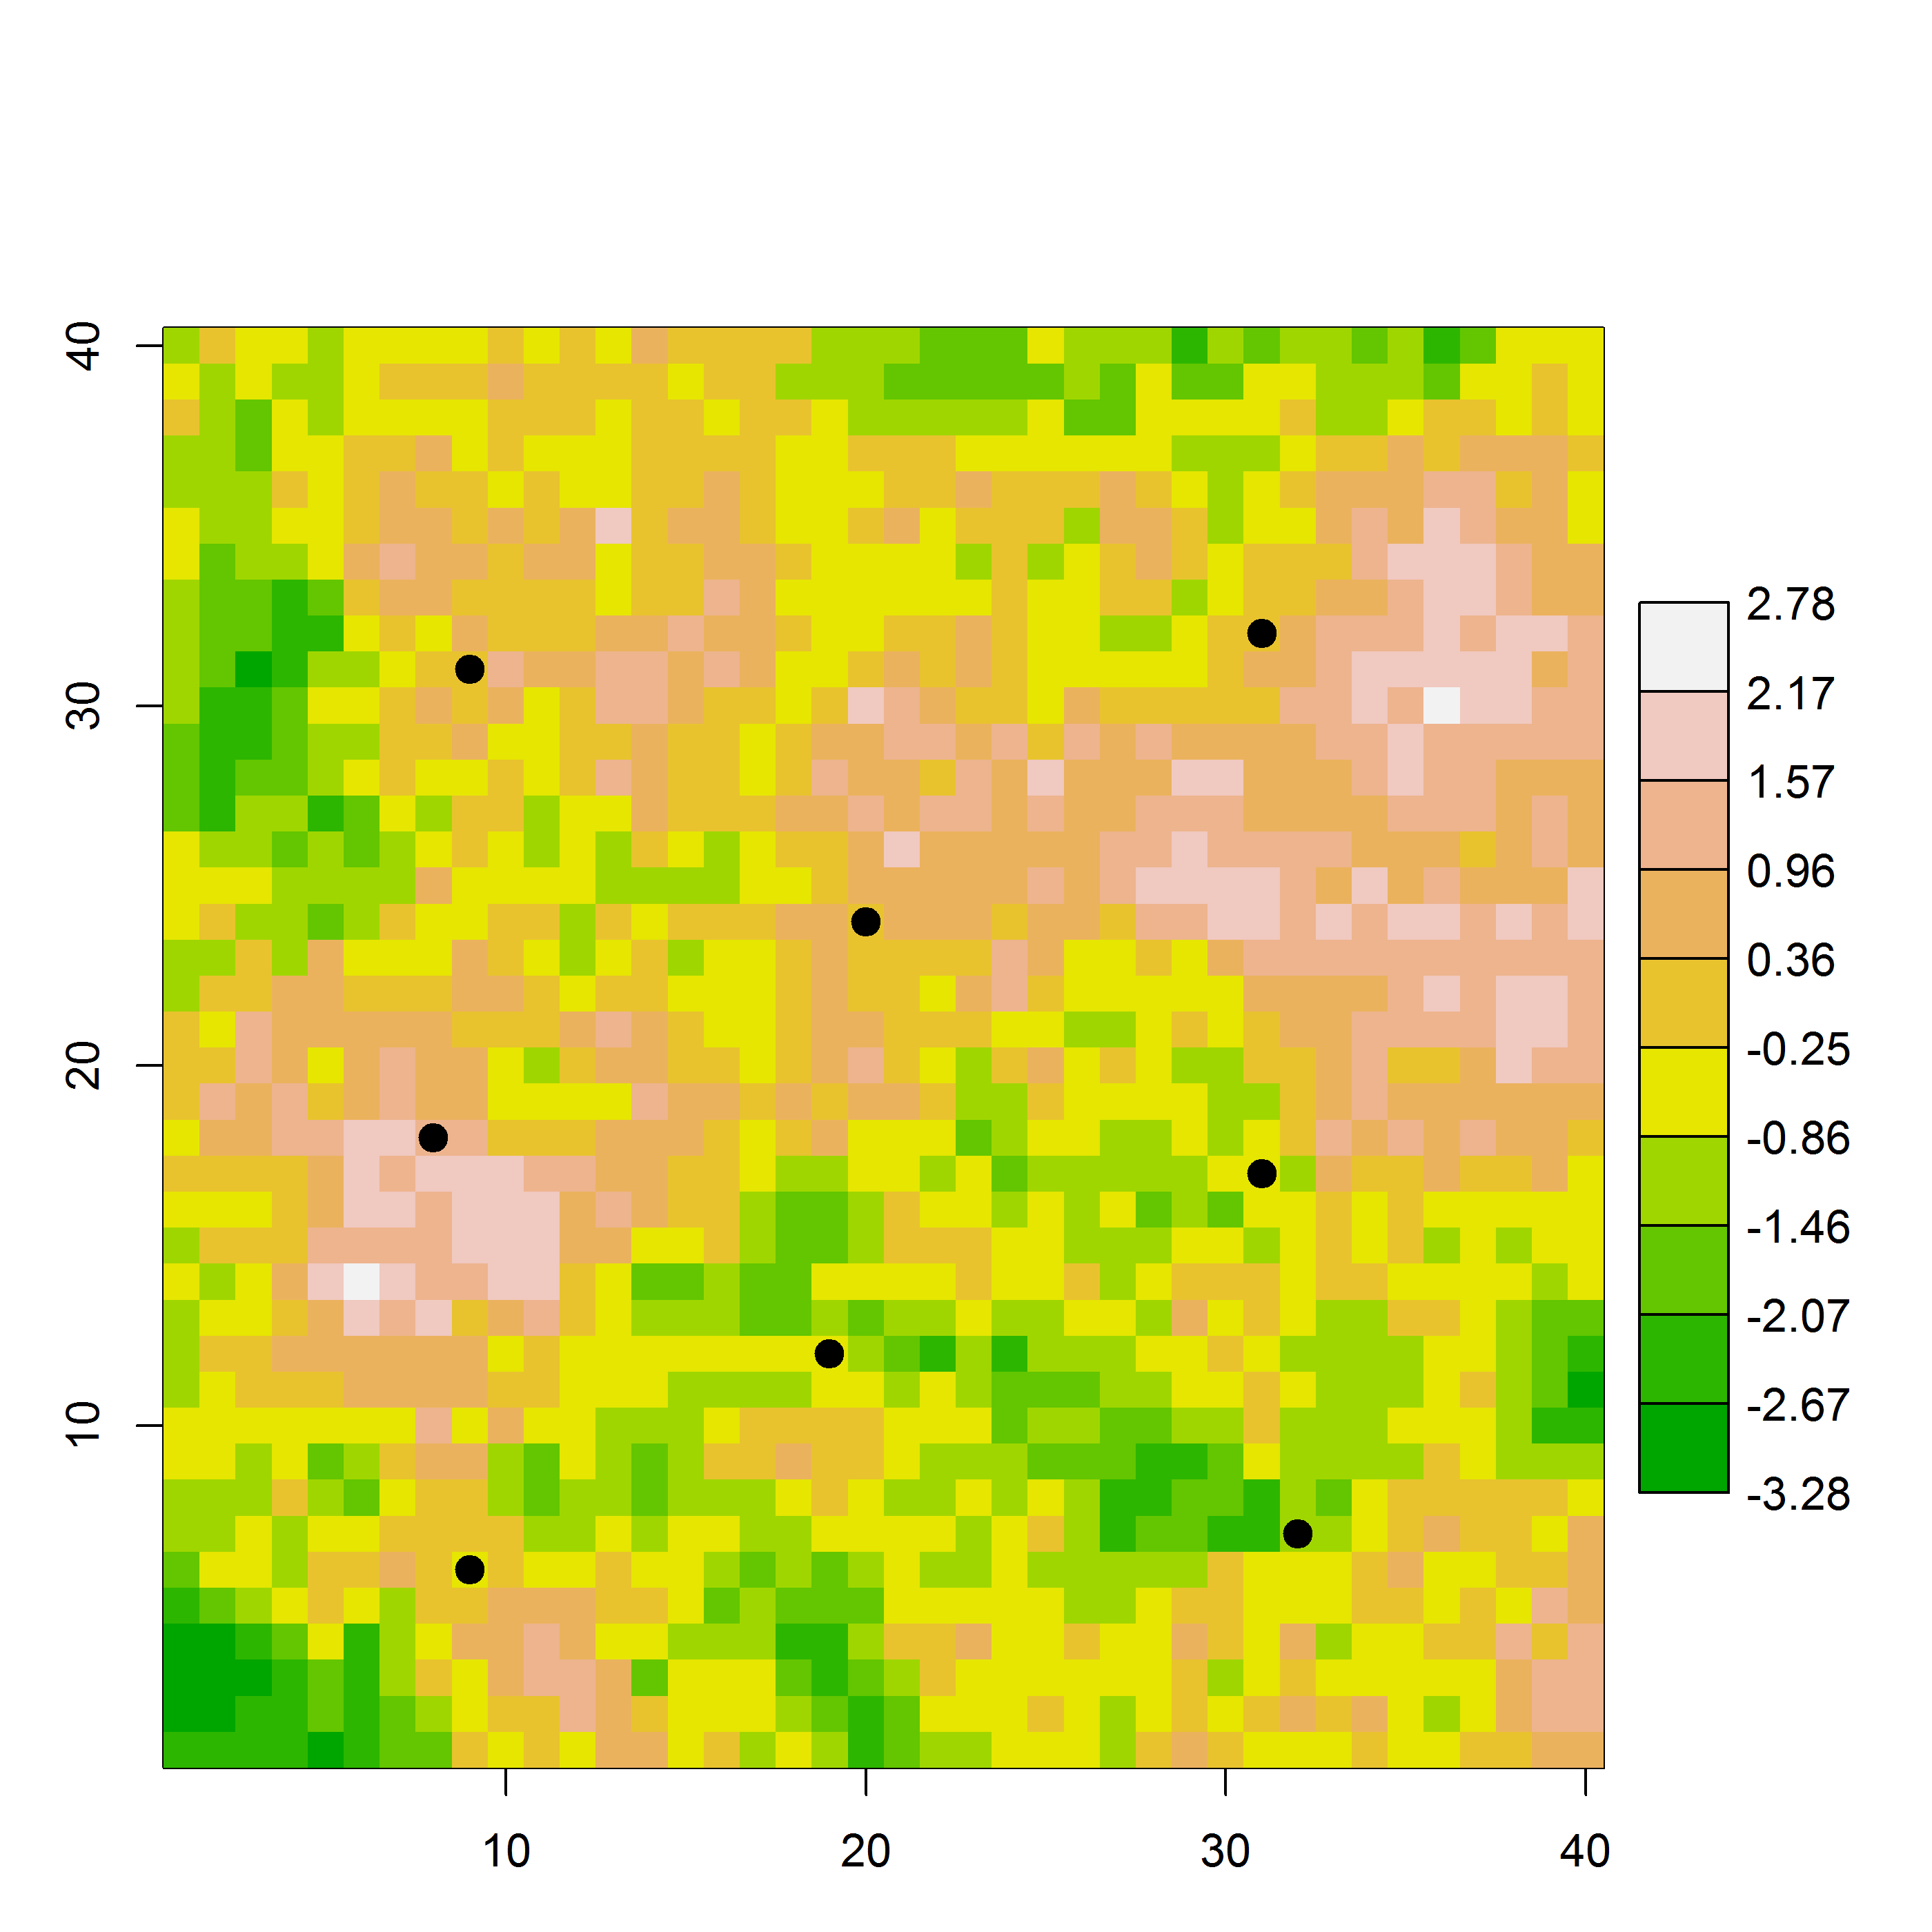
\includegraphics[width=3.5in,height=3.25in]{Ch10-RSF/figs/habitat.png}
\caption{A typical habitat covariate reflecting habitat quality or
  hypothetical utility of the landscape to a species under study. Home range centers for 8 individuals are
shown with black dots.}
\label{rsf.fig.habitat}
\end{figure}
This was simulated by using a
kriging interpolator with the following {\bf R} commands:
\begin{verbatim}
set.seed(1234)
gr<-expand.grid(1:40,1:40)
Dmat<-as.matrix(dist(gr))
V<-exp(-Dmat/5)
z<-t(chol(V))%*%rnorm(1600)
\end{verbatim}
%The functions \mbox{\tt make.statespace} and \mbox{\tt spatial.plot} are
%both in the \mbox{\tt scrbook} package.
Space usage patterns for
 8 individuals are shown in Fig. \ref{rsf.fig.homeranges},
simulated with $\alpha_{1} = 1/(2\sigma^2)$ with $\sigma = 2$ and the
coefficient on $z({\bf x})$ set to $\alpha_{2} = 1$.
\begin{figure}
\centering
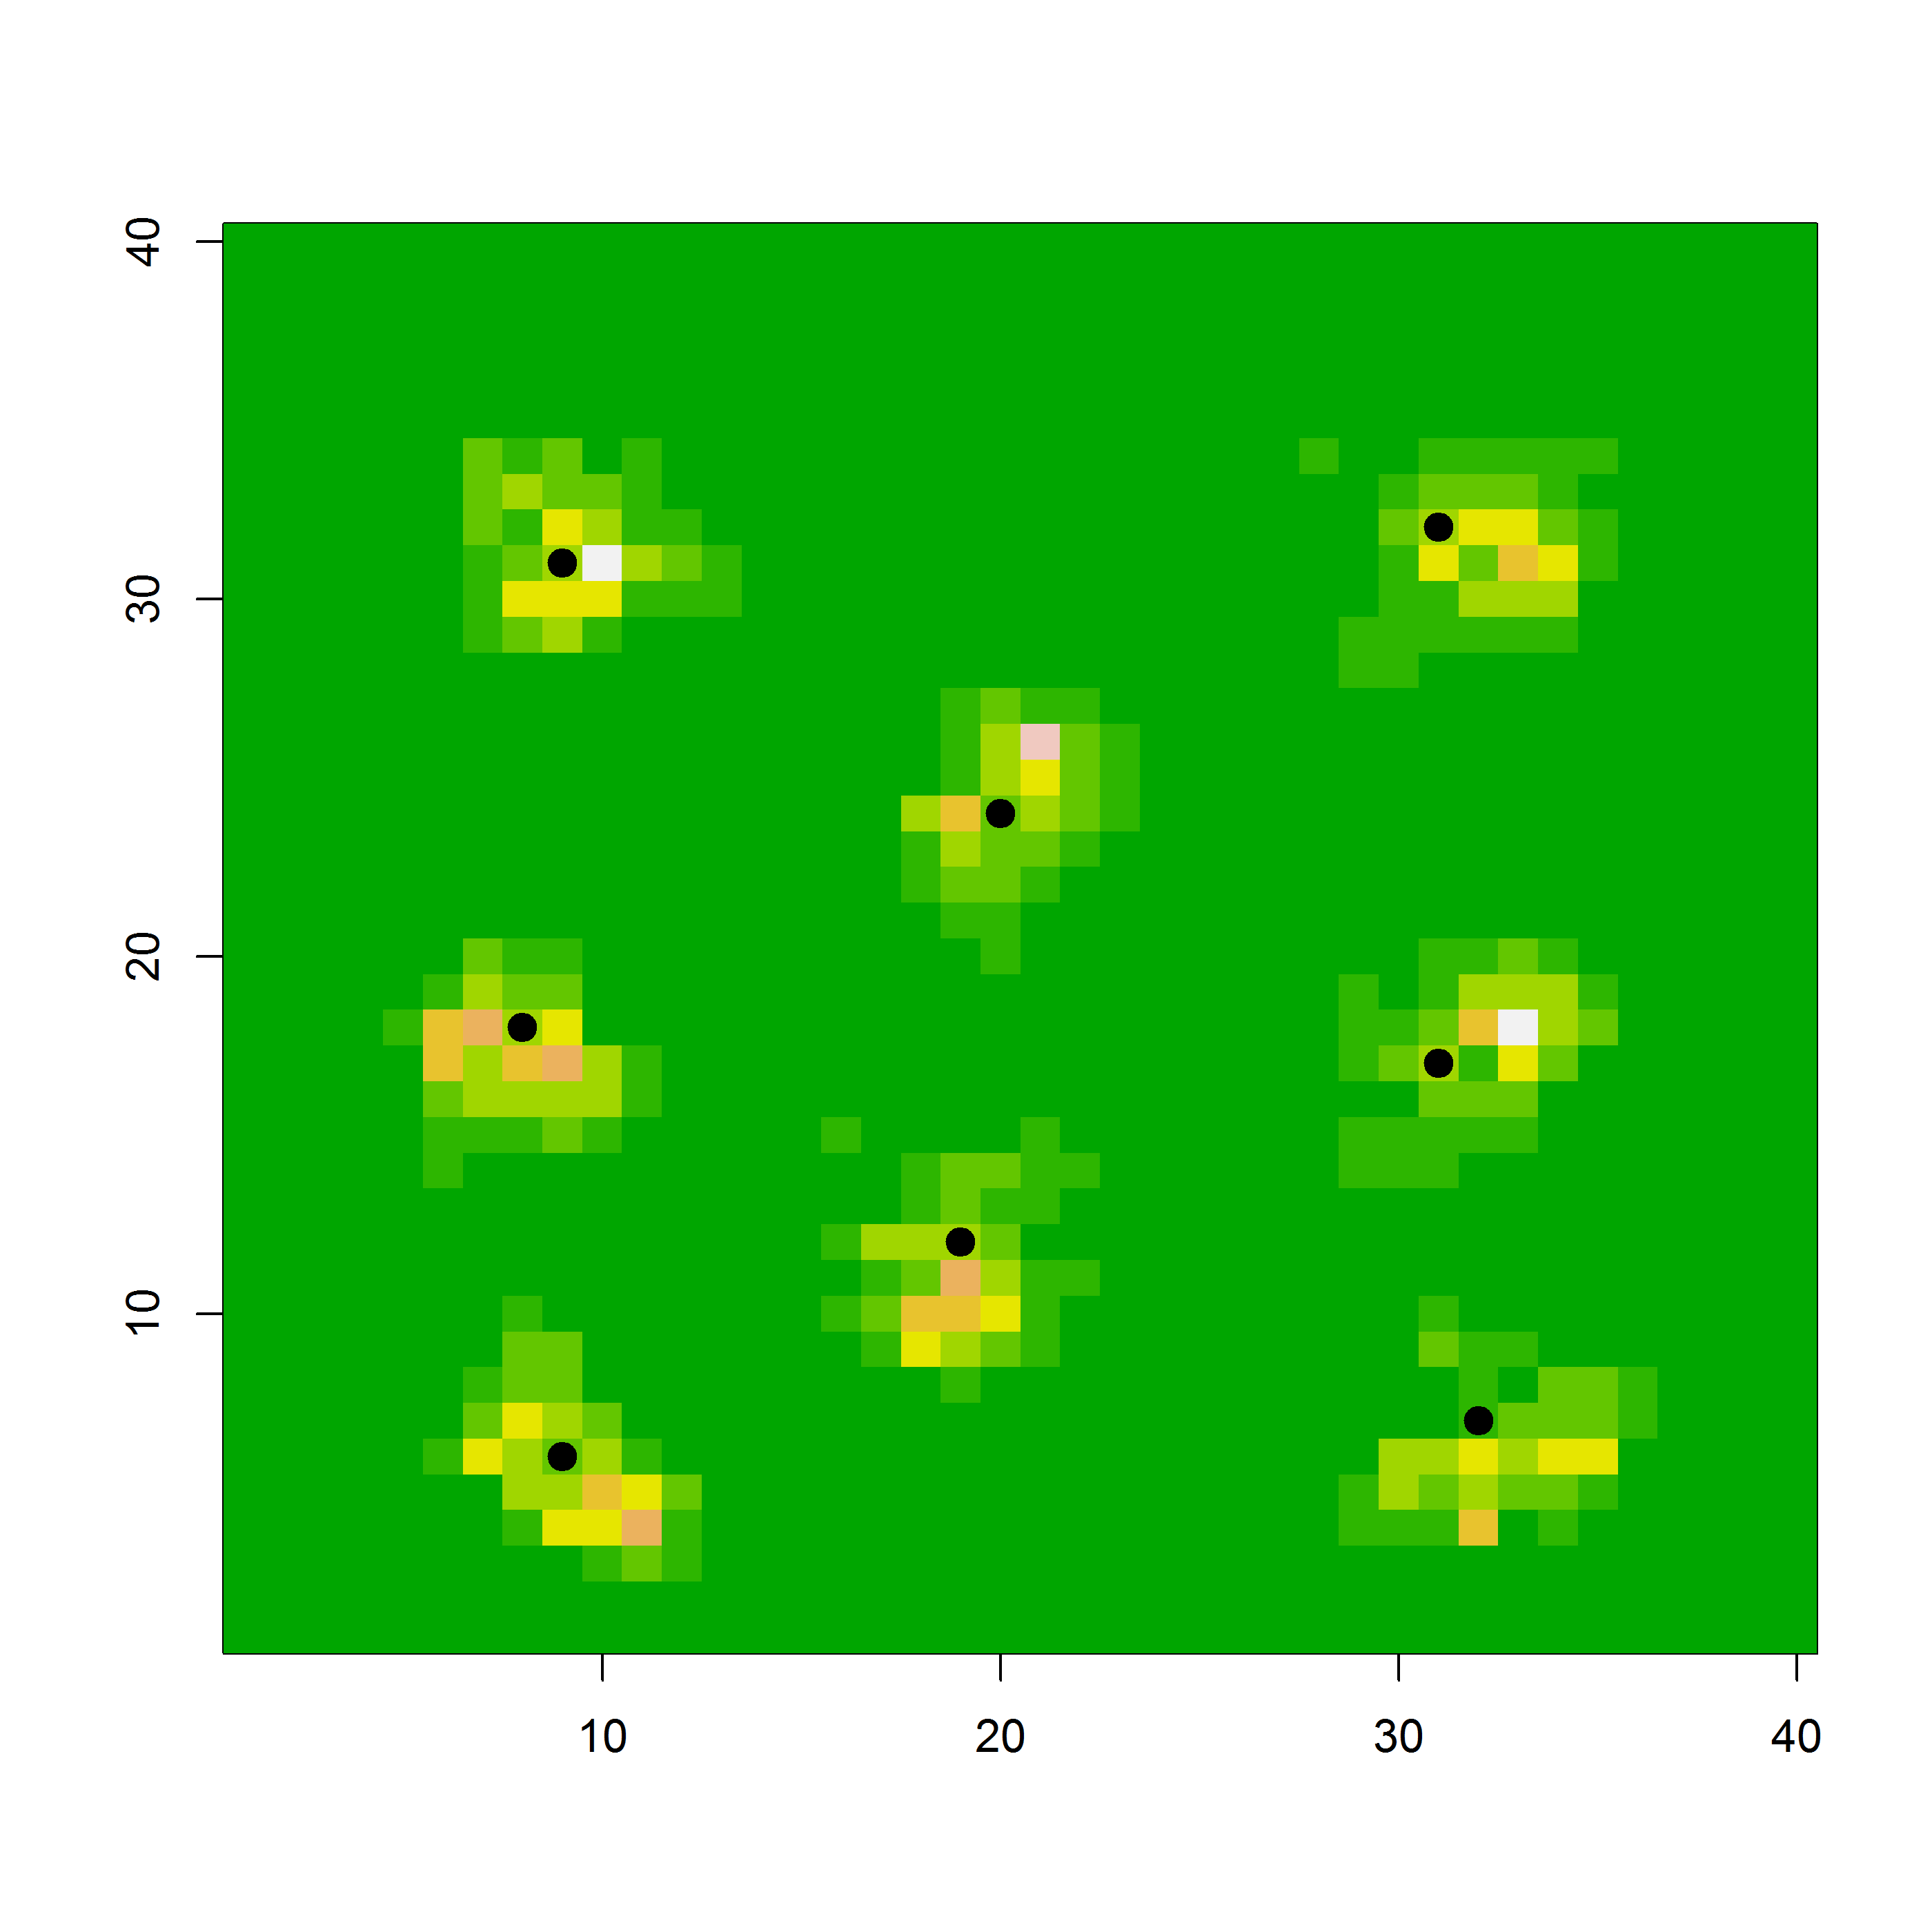
\includegraphics[width=3.5in,height=3.5in]{Ch10-RSF/figs/homeranges8}
\caption{Space usage patterns of 8 individuals under a space usage
  model that contains a single covariate (shown in
  Fig. \ref{rsf.fig.habitat}). Plotted value is the multinomial
  probability $\pi_{ij}$ for pixel $j$ under the model in Eq. \ref{rsf.eq.rsf}.
}
\label{rsf.fig.homeranges}
\end{figure}
These space usage densities -- ``home ranges'' -- exhibit clear
non-stationarity in response to the structure of the underlying
covariate, and they are distinctly asymmetrical.  We note that if
$\alpha_{2}$ were set to 0, the 8 home ranges shown here would
resemble bivariate normal kernels with $\sigma = 2$.  Another
interesting thing to note is that the activity centers are not
typically located in the pixel of highest use or even the centroid of
usage. That is, the observed ``average'' location is not an unbiased
estimator of ${\bf s}$ under the model in Eq. \ref{rsf.eq.rsf}.


\subsection{Poisson use model}

A natural way to motivate the multinomial model of space usage is to
assume that individuals make a sequence of resource selection
decisions so that the outcomes $r_{ij}$ are marginally {\it
  independent}, having a Poisson distribution:
\[
 r_{ij} \sim \mbox{Poisson}( \lambda_{ij})
\]
where
\[
 \log(\lambda_{ij}) = a_{0} -\alpha_{1} D_{ij}^{2} +  \alpha_{2} z({\bf x})
\]
In this case, the number of visits to any particular cell is affected
by the covariate $z({\bf x})$ but has a baseline rate ($\exp(a_{0})$)
related to the amount of movement occuring over some time interval.
This is an equivalent model to the multinomial
model given previously in the sense that, if we condition on the total
sample size $r_{i.} = \sum_{j} r_{ij}$, then the vector ${\bf r}_{i}$
has a multinomial distribution with probabilities
\[
 \pi_{ij} = \frac{\lambda_{ij}}{ \sum_{j} \lambda_{ij}}
\]
which is the same as Eq. \ref{rsf.eq.rsf} (see also
Chapt. \ref{chapt.poisson-mn}) because $a_{0}$ cancels
from the numerator and denominator of the
multinomial cell probabilities
%, analogous to what happens under
%sampling of individual use decisions as discussed above.
and thus this parameter is not relevant to understanding
space usage.

Also note that if use frequencies are summarized over individuals for
each pixel, i.e.,
create the totals $r_j = \sum_i r_{ij}$, then
 a standard Poisson regressino model for the resulting  ``quadrat
 counts'' is reasonable. This is ``Design I'' in \citet{manly_etal:2002}.

\begin{comment}
{\bf note:} while Poisson -> multinomial, it is not vice versa. If the total
sample size per individual is fixed, then the marginals are NOT
Poisson and that model will produce biased estimators.

For purposes of estimation we can use either the Poisson or
multinomial likelihoods. In the former case, we have to estimate an
individual-specific nuisance
parameter $a_{0}$, from which information is derived by the total
number of observations whereas, in the later case, we lose information
about $a_{0}$ by conditioning on the total (i.e., treating it as
fixed).  As it often is fixed, or at least the number of telemetry
observations is completely arbitrary, $a_{0}$ is usually a meaningless
parameter so whether we estimate it or not is immaterial from a
practical standpoint.
\end{comment}





\subsection{Thinning}

Suppose our sampling is imperfect so that we only observe a smaller
number of telemetry fixes than true use, $r_{ij}$. As developed in
sec. \ref{scr0.sec.implied}, we assume that the observed number of
uses is
\[
 m_{ij} \sim \mbox{Bin}(r_{ij}, \phi_{0}).
\]
We can think of these countas as arising by thinning the underlying
point process (here, aggregated into pixels) where $\phi_{0}$ is the
thinning rate of the point process.
In this case, the marginal distribution of $m_{ij}$ is also Poisson
but with mean
\[
 \log(\lambda_{ij}) = \log(\phi_{0}) + a_{0} -\alpha_{1} D_{ij}^{2} +  \alpha_{2} z({\bf x}).
\]
Thus, the space-usage model (RSF) for the
thinned counts $m_{ij}$ is the same as the space-usage model for the
original variables $r_{ij}$.  This is because if we remove $r_{ij}$
from the conditional
 model by summing over its possible values, then the vector of
${\bf m}_{i}$ is {\it also}  multinomial with cell probabilities
\[
\pi_{ij} = \frac{\phi_{0}\lambda_{ij}}{\sum_{j} \phi_{0} \lambda_{ij}}
\]
and so the nuisance parameter $\phi_{0}$ cancels from the numerator and
denominator. Thus, the underlying RSF model applies to the true
unobserved count frequencies ${\bf r}_{i}$ and also those produced
from thinning or sampling, ${\bf m}_{i}$.

%KEY POINT LOST HERE IS THAT BOTH TELEMETRY AND SCR ARE RANDOMLY
%THINNED VERSIONS OF THE POINT PROCESS, PROVIDED CAMERA TRAPPING IS
%RANDOM ALSO

In summary, if we conduct a telemetry study we observe ${\bf r}_{i}$,
the $nG \times 1$ vector of pixel-counts for each individual
$i=1,\ldots,N_{tel}$.  We declare these data to be
``resource-selection data'' which are typical of the type used to
estimate resource-selection functions (RSFs) \citep{manly_etal:2002}.
Sometimes in RSF modeling activities we might have
continuous covariates and so the denominator in Eq. \ref{rsf.eq.rsf}
involves an integration over a distribution for the covariate which is
the conditional intensity of observed point locations in a point
process model. However, in a discrete landscape, entertaining pdfs for
the covariates isn't necessary \citep{royle_etal:2012mee} when we
recognize that the denominator should be the expectation over {\it
  space} and not the pdf of some covariate.


\subsection{Capture-recapture Data}

XXXXXXXXXXXXXXXXXXX
RC says: After reconciling SCR and RSF, cite that paper
by Boyce and McDonald where they try to do accomplish the same
objective using ad-hoc methods. That is the only effort to do
something similar that I am aware of.
XXXXXXXXXXXXXXXXXXXXXXXXXX

The key to combing RSF data with SCR data is to work with this
underlying resource utilization process and formulate SCR models in
terms of that process. The idea in \citep{royle_etal:2012mee} was to
define the true use frequency for each pixel as 
the intermediate latent variable to which both telemetry data and SCR
data are linked.
Obviously we have to assume that both telemetered individuals
and SCR individuals are using space according to the same resource
selection model. The difference is that, for SCR data, we do not have
sampling devices in all locations (pixels) in the landscape, and hence
the data are only recorded at a subsample of them. XXXXX {\bf move the
  following } XXXXX
In other words,
imagine that we have a sampling device, such as a camera trap, in {\it
  every} pixel. If the device operates continually then it is no
different from a telemetry instrument.  If it operates intermittently
and does not expose the entire area of each pixel then a reasonable
model for this imperfect observation is the ``thinned'' binomial model
given above, where $\lambda_{0} \equiv \exp(\phi_{0})$ represents the
sampling effectiveness of the device. So we imagine that the
hypothetical perfect data from a camera trapping study are the thinned
counts $m_{ij}$ for every pixel $j$.

Introducing the latent use
 frequencies $m_{ij}$, and considering the Bernoulli SCR model
where
$y_{ij} = 1$  if the individual $i$ visited the pixel
containing a trap and was detected, then
we imagine that $y_{ij}$ is related to the latent variable $m_{ij}$ being the
event $m_{ij}>0$, which occurs with probability
\[
 p_{ij} = 1-\exp(- \lambda_{ij})
\]
where
\[
 \log(\lambda_{ij}) = \log(\phi_{0}) + a_{0} -\alpha_{1} D_{ij}^{2} +  \alpha_{2} z({\bf x}).
\]
We combine the constants so that $\alpha_{0} = \log(\phi_{0}) + a_{0}$
is the baseline encounter rate which includes the constant intensity
of use by the individual and also the baseline rate of detection,
conditional on use.  The Bernoulli observation model implies that the
observed encounter frequencies for individual $i$ and trap $j$, from
sampling over $K$ encounter periods is:
\[
 y_{ij}|{\bf s}_{i} \sim \mbox{Bin}(K; p_{ij})
\]
We imagine that any of the standard SCR observation model could be
implemented here with only minor modifications of the encounter
probability model (following the developments of Chapt. \ref{chapt.poisson-mn}.


\section{The Joint RSF/SCR Likelihood}

To construct the likelihood for SCR data when we have auxiliary
covariates on space usage {\it or} direct information on space usage
from telemetry data, we regard the two samples (SCR and RSF) as
independent of one another. In practice, this might not always be the
case but (1) often time the telemetry data come from a previous study;
(2) the individuals are not the same at all; (3) or even if they are
some of the same individuals being captured, we might not be able to
match individuals captured by a sampling method such as hair-snares
with the individuals wearing radio-collars; (4) In cases where we {\it
  can} match some individuals between the two samples, regarding them as
independent should only entail a minor
loss of efficiency
because we are disregarding more precise information on a small number
of activity centers. Moreover, we believe, it is unlikely in practice
to expect the two samples to be completely reconcilable and that the
independence formulation is the most generally realistic.

Regarding the two data sets as being independent, our approach here
is to form the likelihood for each set of observations as a function
of the same underlying parameters and then combine them. In
particular, let ${\cal L}_{scr}(\alpha_{0}, \alpha_{1}, \alpha_{2}, N;
{\bf y}_{scr})$
be the likelihood for the SCR data in terms of the basic encounter
probability parameters and the total (unknown) population size $N$,
and let ${\cal L}_{rsf}(\alpha_{1},\alpha_{2}; {\bf m}_{rsf})$ be the
likelihood for the RSF data based on telemetry which, because the
sample size of such individuals is fixed, does not depend on $N$.
Assuming independence of the two datasets, the
joint likelihood is the product of these two pieces:
\[
{\cal L}_{rsf+scr}(\alpha_{0},\alpha_{1},\alpha_{2},N; {\bf y}_{scr},{\bf
  m}_{rsf})  = {\cal L}_{scr} \times {\cal L}_{rsf}
\]
In what follows, we provide a formulation of each likelihood
component, along with an {\bf R} function for obtaining the MLEs of
model parameters using standard methods available in {\bf R}.


Where the L(scr) is the normal integrated likelihood (chapt XXX,
equation XXXX) and the rsf likelihood is the multinomial telemetry
likelihood from eq. XXXX above. 
That is, if we estimate s for the telemtered guys by the mean location
then we could use that plug-in otherwise we also have to inegrate the
multnomial likelihood ..........
For the RSF data from the sample of individuals with telemetry devices
we adopt the same basic strategy of describing the
conditional-on-${\bf s}$ likelihood and then computing the marginal
likelihood by averaging over possible values of ${\bf s}$.
We have ${\bf m}_{i}$, the vector of pixel counts for individual $i$,
where these counts are derived from a telemetry study or similar.
The conditional-on-${\bf s}_{i}$ distribution of the telemetry data
from individual $i$ is:
\[
 [{\bf m}_{i}  | {\bm \alpha} ]
 = \prod_{g=1}^{G}  \pi_{ij}({\bf s}_{i},z({\bf x}_{j})) ^{r_{ij}}
\]
where
\[
 \pi_{ij}  = \frac{ \exp( -\alpha_{1} D_{ij}^{2} +\alpha_{2} z({\bf x}_{j}) ) }
{ \sum_{g} \exp(-\alpha_{1} D_{ij}^{2} +\alpha_{2} z({\bf x}_{j}))}
\]
The marginal pmf is:
\[
     [{\bf m}_{i}|{\bm \alpha}] =    \int_{{\cal S}}  [ {\bf m}_{i} |{\bf s}_{i},{\bm \alpha}] g({\bf s}_{i}) d{\bf s}_{i}
\]
and therefore the likelihood for the RSF data is
\[
{\cal L}_{rsf}({\bm \alpha} | {\bf m}_{1},{\bf m}_{2},\ldots, {\bf m}_{Ntel}) = \prod_{i=1}^{Ntel}
[{\bf m}_{i}|{\bm \alpha}].
\]

An R script is given in \mbox{\tt scrbook} which is the function XXXX
from manuscript ADD TO REPO XXXXXX... will handle estimated s by sbar
or whatever.   Should be obvious that estimating s with sbar is not
the greatest thing because there is a covariate affecting use, and so
we expect the geographic centroid to be biased for s.



\section{Application: New York Black Bear Study}
\label{rsf.chapt.nybears}


\citet{royle_etal:2012mee}
applied the integrated SCR+RSF model to data from a study of black bears in a
region of approximately 4,600 km$^2$ in southwestern New York
\citep{sun:2013}. We reproduce their results here.
The data can be loaded from the \mbox{\tt scrbook} library with the
command \mbox{\tt data(nybears)}. {\bf XXXX do this on the repo XXXXX}
A noninvasive, genetic, mark-recapture
study was conducted to estimate density, and a concurrent telemetry
study was conducted in the same study area to understand patterns of
landscape connectivity and space usage.
The study used DNA sampling obtained from 103
hair snares 
(Fig. \ref{rsf.fig.studyarea})
set  from 6 June - 9 July, 2011.
Hair snares
were baited and scented and checked weekly for hair. 
See \citet{sun:2013} for details of the genetic analysis.

The study yielded
captures of 33 individuals and a total of 14 recaptures (27
individuals captured 1 time only; 3 individuals captured twice; 1
individual each three and four times). Extra trap recaptures included
3 individuals captured in 2 traps, 1 individual in each of 3 and 4
traps.  We used data from 3 radio-telemetered individual bears (2M,
1F) from the same time period as the SCR data. Radio fixes were
obtained approximately once per hour and a total of 1,948 fixes on the
3 individuals were obtained. We thinned these hourly fixes to once per
10 hours to approximate the data as independent movement outcomes,
producing 195 telemetry locations used in the RSF component of the
model.  We used the covariate elevation in the model, derived from a
one arc-second digital elevation model (USGS National Elevation
Dataset, accessed June 2012).  This is shown in
Fig. \ref{fig.elevation} (on a
standardized scale) which also shows the locations of each capture
(multiple captures at a trap location are dithered by adding random
noise).


We fitted a sequence of models based on the Gaussian hazard model
(eq. \ref{eq.hazard})  including an ordinary SCR model with no
covariates or telemetry data, the SCR model with elevation affecting either
$\lambda_{0}$ or density $D({\bf x})$, and models that use telemetry data. We have not discussed modeling
covariate effects on density, but such models are described by
\citet{borchers_efford:2008} and we have not provided any novel
treatment of that modeling aspect here.
The full list of models (with labels) is as follows:
\begin{itemize}
\item[] Model 1: SCR -- ordinary SCR model
\item[] Model 2: SCR+p(z) -- ordinary SCR model with elevation as a
  covariate on baseline encounter probability $\lambda_{0}$.
\item[] Model 3: SCR+D(z) -- ordinary SCR model with elevation as a
  covariate on density only.
\item[] Model 4: SCR+p(z)+D(z) -- ordinary SCR model with elevation as
  a covariate on both baseline encounter probability and density.
\item[] Model 5: SCR+p(z)+RSF -- SCR model including data from 3
  telemetered individuals.
\item[] Model 6: SCR+p(z)+RSF+D(z) -- SCR model including telemetered
  individuals and with elevation as a covariate on density.
\end{itemize}
The first 4 models can be viewed together for purposes of
model-selection by AIC since they are nested models. The last two
models can be viewed together but cannot be compared to the first 4
because they include telemetry data.
The results of fitting these 6 models -- the parameter estimates and
standard errors are shown in Table \ref{tab.nyresults}.
We provide a full R script for fitting  all of these models to
simulated data in Appendix 1.


Among models 1-4, those models {\it without} the telemetry data, we
see that the two models with elevation affecting density are preferred
-- and, there is a large positive response to elevation. This is
consistent with the visual pattern apparent in
Fig. \ref{fig.elevation} where we see individual captures favoring
high elevation sites.  We also see a negative effect of elevation on
{\it space usage} (the parameter $\alpha_{2}$).  It is interesting
that the sign of the estimate of $\alpha_{2}$ changes from positive to
negative when we add elevation as a covariate on density. Thus, the
effect of elevation on density appears to have masked its effect on
space usage.  The estimate of $N$ for the 4600 km$^2$ state-space is
about 103 bears $(\exp(4.25)+33)$.

In the two models that include the additional telemetry data, a couple
points stand out: Clearly the elevation effect on density is
important, reducing the negative log-likelihood by 5 units. The effect
of elevation on density and space usage are roughly consistent with
Model 4 which did not use telemetry data. Furthermore, the standard
errors (SE) of those two parameter estimates are reduced considerably
when the model uses telemetry data, as is the SE for estimating
$\log(\sigma)$.  The SE for estimating $\log(n_{0})$ is only improved
incrementally compared to the models without telemetry data.  We used
the best model, \mbox{\tt SCR+p(z)+RSF+D(z)}, to produce a map of
density (Fig. \ref{fig.density}) which shows clearly the pattern
induced by elevation. We also produced a map
(Fig. \ref{fig.spaceusage}) to illustrate the effect of elevation on
space usage. This shows the relative probability of using a pixel
${\bf x}$ relative to one of mean elevation, and of the same distance
from an individual's activity center.
% remind people how to compute "the relative prob of using pixel x XXXX
%The cool thing about these models is we can make pretty
%multi-colored maps of things.  A map of density under the 
%model is shown in fig. \ref{fig.density}.  A map of space usage in
%terms of the relative probability of using pixel $x$ relative to the
%average pixel is shown in Fig. \ref{fig.spaceusage}.


% XXXX should we add AIC to this table? XXXX
\begin{table}
\centering
\caption{
Summary of model-fitting results for the black bear study. Parameter
estimates are $\alpha_{0} = \log(\lambda_{0})$ and $\sigma$ is the
scale parameter of the half-normal hazard rate encounter model.
The SCR data are based on $n=33$ individuals, and the telemetry data
are based on 3 individuals.
}
\begin{tabular}{c|rrrrrr}
\hline \hline
model & $\alpha_0$ & $\log(\sigma)$ & $\alpha_{2}$ & $\log(n_{0})$ &
$\beta$ & -loglik \\ \hline
SCR+p(z)     & -2.8600  & -1.1170  &  0.1750 &  4.1400   &        &122.7380  \\
   SE        &  0.3899 &  0.1390 &  0.2478&  0.3657  &        & \\
 SCR         & -2.7290  &  -1.1220 &  ---&  4.1100   &        &              122.9900   \\
   SE        &  0.3454 &   0.1404&        &  0.3618  &        &       \\
SCR+D(z)     & -2.7150  & -1.1330  &  ---  &  4.1140   & 1.2470  &   118.0070  \\
   SE        &  0.3526 & 0.1394  &        &  0.3575  & 0.4083 &       \\
SCR+p(z)+D(z)& -2.4840  & -1.1570  &-0.3840  &  4.2550   & 1.5710  &      117.0750 \\
   SE        &  0.3910 &  0.1421 & 0.2761 &  0.3768  & 0.4630 & \\
SCR+RSF     &   -3.0680  & -0.8140  &-0.2810  &  3.8840   &        &   1271.7390 \\
   SE       &    0.2722 &  0.0364 & 0.1176 &  0.3626  &        & \\
SCR+RSF+D(z)&  -3.0700  &-0.8100   &-0.3710  &  4.0280   & 1.2730  &   1266.7000 \\
   SE       &   0.2720 &  0.0368  & 0.1239 &  0.3661  & 0.4110 &    \\
\hline
\end{tabular}
\label{tab.nyresults}
\end{table}





Resource selection can be described in
hierarchical orders \citep{johnson:1980}, from selection of a geographical
area (first-order selection), selection of a home range within a study
area (second-order), or selection of resources with that home range
(third-order).  Animals may select resources at different scales as a
result of variability in the distribution of resources on the
landscape \citep{mayor_etal:2009}.  Indeed, black bears make habitat
selection decisions at multiple spatial scales, and decisions made at
the second-order can differ from those at the third-order
\citep{lyons_etal:2003, sadeghpour_ginnett:2011}.
  As a result of multi-scale
resource selection, we can expect that the modeled covariates
(elevation in our example) may affect density and space usage
differently.  We suggest that density is operating at the second-order
and is largely related to the spacing of individuals and their
associated home ranges across the landscape.  On the other hand, our RSF was defined
based on selection of resources within the home range (third-order).
Because density and our third-order RSF were at different spatial
scales, there is no expectation that the modeled covariate describing
space usage (elevation) would influence each in a similar manner.
Consistent with our positive relationship between elevation and
density, the distribution of a black bear population in the central
Appalachian Mountains was positively associated with elevation \citep{frary_etal:2011}.
 At the second-order, however, we observed a negative
effect of elevation on space usage.  Our study was conducted during
summer, and seasonal shifts in elevation have been widely documented
in black bears, often attributed to seasonal variation in food
availability \citep{reynolds_beecham:1980,
%garshelis_pelton:1981,kendall:1983, 
graber_white:1983}.
%%irwin_hammond:1985, raine_kansas:1990}.
 The negative relationship between elevation and space
usage during the summer could be attributable to either access to food
resources at lower elevations, or access to river and stream
corridors.  Within their home ranges, black bears selected areas with
high stream densities \citep{fecske_etal:2002}, and in our study area,
lower elevations were associated with river corridors which likely
provided bears cooler conditions during the heat of summer.





\section{Simulation Study}

Royle et al. XXXXX 
 carried-out a simulation study using the landscape shown in
Fig. \ref{rsf.fig.habitat}, and based on a population of $N=100$ and $N=200$
individuals with activity centers distributed uniformly over the
landscape.  This patchy covariate was simulated by generating a field
of spatially correlated noise to emulate a typical patchy habitat
covariate such as tree or understory density, or some other covariate
relevant to habitat quality for a species.  We subjected individuals
to sampling over $K=10$ sampling periods, using a $7 \times 7$ array
of trapping devices located on the the integer coordinates $(u*5,v*5)$
for $u,v = 1,2,3,4,5,6,7$. The model parameters were
\[
\mbox{ cloglog}(p_{ij}) = -2  -\frac{1}{2\sigma^{2}} D_{ij}^{2} + 1 \times z({\bf x}_{j})
\]
for $\sigma =2$. In the absence of the covariate $z$, this corresponds
to an individual having a bivariate normal home range with standard
deviation 2.
These settings yielded an average of about $n=61$ individuals captured for
the $N=100$ case and about $n=123$ for the $N=200$ case. The later case
represents what we believe is an extremely large sample size based on
our own experience and thus it should serve to gauge the large sample
bias of the likelihood estimator (note: we expect little to no large
sample bias).

In addition to simulating data from this capture-recapture study, we
simulated 2, 4, 8, 12, 16 telemetered individuals to assess the
improvement in precision as sample size increases.  For all cases we
observed 20 telemetry fixes {\it per} individual.  The main things
we're focused on with this simulation study were: (1) how much does
the SE of estimated $N$ improve as we add or increase the number of
telemetered individuals?  (2) How well does the SCR model do at
estimating the parameter of the RSF with {\it no} telemetry data?  (3)
How much does the precision of the RSF parameter improve if we add SCR
data to the telemetry data?


%% Should also simulate fitting the wrong model with symmetric
%% encounter model and see what happens
%% also run N=200 with 500 iterations

{\small
\begin{verbatim}
N=100, 300 iters each, mean SCR only N: 99.418     N=200, 500 iters. Mean SCR only N = 199.712
n=2          Nhat RMSE  ahat RMSE  sighat  RMSE    Nhat RMSE  ahat RMSE  sighat  RMSE
SCR only:   99.73  9.97  0.99  0.14  2.00  0.124  198.85  14.24   0.99   0.10   2.00   0.091
SCR/RSF:    99.94  9.54  0.99  0.12  2.00  0.097  199.37  12.80   0.99   0.09   2.00   0.078
sbar        98.89  9.50  0.93  0.14  1.97  0.100  197.87  13.94   0.96   0.10   1.99   0.080
RSF only     --    --    1.03  0.33  2.00  0.160    --      --    1.04   0.33   1.99   0.169
n=4
SCR only    99.10  9.83  0.99  0.13  2.00  0.127  200.06  15.34   1.00   0.09   2.00   0.092
SCR/RSF     99.17  9.47  0.99  0.11  2.00  0.086  200.25  14.36   1.00   0.08   2.01   0.073
sbar        97.43  9.68  0.89  0.16  1.97  0.090  198.14  14.31   0.94   0.10   1.98   0.075
RSF only     --     --   0.98  0.22  2.00  0.119    --     --     1.02   0.21   2.01   0.122
n=8
SCR only    99.59 10.00  1.00  0.13  2.00  0.130  200.85  14.06   1.00   0.09   2.00   0.087
SCR/RSF     98.90 10.02  0.99  0.10  2.00  0.071  200.29  13.98   1.00   0.08   2.00   0.061
sbar        96.07 10.37  0.84  0.19  1.96  0.078  196.46  14.59   0.90   0.13   1.97   0.069
RSF only     --    --    0.98  0.16  2.01  0.084    --     --     0.99   0.16   2.00   0.084
n=12
SCR only    99.44 10.73  0.98  0.13  2.02  0.128  198.76  14.47   0.99   0.10   2.00   0.091
SCR/RSF     99.96 10.26  1.00  0.09  2.00  0.059  198.72  14.14   1.00   0.08   2.00   0.054
sbar        96.30 10.49  0.82  0.20  1.96  0.071  193.83  15.14   0.87   0.15   1.97   0.063
RSF only     --    --    1.01  0.12  2.00  0.069    --     --     1.01   0.13   2.00   0.069
n=16
SCR only    99.23 10.74  0.99  0.14  2.00  0.128  200.04  14.09   0.99   0.10   2.01   0.088
SCR/RSF     99.20  9.79  1.00  0.09  1.99  0.057  200.25  13.40   1.00   0.07   2.00   0.047
sbar        95.10 10.17  0.80  0.22  1.95  0.075  194.38  14.26   0.85   0.17   1.96   0.059
RSF only     --    --    1.00  0.10  1.99  0.061    --     --     1.00   0.11   2.00   0.055

To check misspecification with isotropic h/r model I refitted the N =
200 cases and fit the SCR only and SCR/RSF models IN ADDITION to the
SCR0 model with isotropic encounter model.
n=2
SCR only 199.11  14.28   0.99   0.09   2.00   0.090
SCR/RSF  199.11  13.80   0.99   0.09   2.00   0.079
SCR0     161.48  39.98    --     --    1.84   0.180

n=4
SCR only 199.67  13.87   1.00   0.09   2.00   0.090
SCR/RSF  199.65  13.59   1.00   0.09   2.00   0.072
SCR0     161.32  40.00    --     --    1.83   0.191

n=8
SCR only 199.24  15.49   0.99   0.10   2.01   0.093
SCR/RSF  199.55  14.17   0.99   0.08   2.00   0.063
SCR0     161.46  40.06    --     --    1.84   0.184

n=12
SCR only 200.41  15.16   0.99   0.10   2.00   0.086
SCR/RSF  200.95  13.04   1.00   0.08   2.00   0.051
SCR0     162.40  38.95    --     --    1.84   0.185

n=16
SCR only 199.16  15.62   1.00   0.09   2.00   0.095
SCR/RSF  199.63  13.38   1.00   0.07   2.00   0.052
SCR0     160.93  40.44    --     --    1.84   0.190
\end{verbatim}
}


The replicate runs of the SCR-only situation give us an idea of the
inherent MC error in these simulations, which is roughly about
0.25 and 0.89 on the $N$ scale for the $N=100/N=200$ cases.
 The mean $N$ under ``\mbox{\tt SCR only}''
across all 5 simulations for $N=100$ was $\mbox{mean}(\hat{N}) = 99.418$, an empirical bias of
$0.6\%$. For N=200, the estimated $N$ across all 5 simulations (5
levels of ntel)  was
$\mbox{mean}(\hat{N}) = 199.712$, an empirical bias of about $0.15\%$, within the MC error of
the true value of $N=200$.
The results suggests a very small bias of $< 1\%$
in the MLE of $N$ in general when estimation is based on the full
marginal likelihood. However, there is apparent bias of as much as 2-4\% when ${\bf s}$ is
estimated by the average observed location.
The bias is slightly
diminished  as we double the expected sample size by doubling $N$ from 100 to
200.
  In practice, we expect a
small amount of bias in MLEs as likelihood theory only guarantees
asymptotic unbiasedness.
 Moreover, the landscape resolution is fairly coarse relative
to $\sigma$ in our study, having a 1 km resolution whereas $\sigma =
2$, which we expect to introduce a small amount of negative bias
because it is an explicit under-statement of the true heterogeneity in
$p$ due to the spatial context of the problem.  The apparent bias that
arises as a result of esetimating ${\bf s}$ is expected because the
average location of an individual would be unbiased for ${\bf s}$ only
if the individual is moving according to a stationary isotropic
kernel. Under the model of space usage with covariate $z({\bf x})$,
then the average location is biased to favor good values of $z({\bf
  x})$ and so $\bar{\bf s}$ is really biased for ${\bf s}$.
%%%% XXXX \hl{again,  is there an unbiased estimator available?}
%%%% Good question -- probably
%%% Let us put that on the "to do" list


In terms of RMSE of the MLEs, generally there is about a 5\% reduction
in RMSE when we have at least 2 telemtered individuals,
and, although
there is a lot of MC error in the RMSE quantities, it might be as much
as a 10\% reduction (tops) as $n$ increases under the higher $N=200$ setting. This makes sense because
we nail down the parameters and still don't know where guys are, and
get info about mean p, i.e. $\alpha_{0}$, only from the SCR data. Thus
estimating $N$  benefits only slightly from the addition of telemetry
data.
%\hl{I don't understand how this could be true. It seems like
%  there should be a tight relationship between the uncertainty about
%  $sigma$ and that of $N$?? That is what we found when we used the
%  informative prior in our AOAS paper.}

Estimating the RSF parameter $\alpha_{2}$ exhibits negligible or no
bias except when ${\bf s}$ is estimated and, interestingly, it is
well-estimated from SCR data alone and even better than RSF data alone
(in terms of RMSE) until we have more than 200 or so telemetry
observations.  The big improvement comes in esetimating the home range
parameter $\sigma$ which is unbiased except when we estimate ${\bf s}$
in which case it exhibits only modest bias.  However, there is huge
improvement in RMSE of $\hat{\sigma}$, perhaps as much as 50-60\% in
some cases, but that really doesn't translate much into esetimating
$N$.  Improvement due to adding RSF data from telemetry diminishes as
the expected sample sizes increases, and so telemetry data does less
to improve the precision of
%has less affect at improving the precision of
$\hat{\sigma}$ and $\hat{\alpha}_{2}$
for $N=200$ than for $N=100$.

We simulated a low $p$ situation in which $\alpha_{0}=-3$ producing
$E[n] = 37$ under the $N=100$ scenario.  The effect is we have only
incremental relative improvements in RMSE of $N$ but relatively more
improvement in RMSE for estimating $\sigma$. The MLE of
$N$ is positively biased.
% remove this in the manuscript
Interestingly this bias opposes slightly negative bias for
the estimator based on estimating ${\bf s}$ and so that the wrong
estimator actually does better. This is a complete chance occurrence
and we should not get too excited by that.
{\small
\begin{verbatim}
N=100, low p, 500 iterations
n=2        Nhat   RMSE   ahat  RMSE   sighat  RMSE
SCR only 103.85  22.88   1.00   0.19   2.02   0.261
SCR/RSF  102.90  20.98   1.00   0.17   2.00   0.136
sbar     101.55  20.91   0.90   0.19   1.96   0.136
RSF only   --     --     1.02   0.30   1.99   0.163
n=4
SCR only 105.65  26.52   1.01   0.20   2.01   0.258
SCR/RSF  103.55  22.92   1.01   0.14   2.00   0.104
sbar     100.86  22.57   0.86   0.20   1.95   0.113
RSF only   --     --     1.01   0.21   1.99   0.114
n=8
SCR only 107.41  45.05   0.99   0.19   2.01   0.254
SCR/RSF  104.28  22.13   1.00   0.12   2.00   0.076
sbar      99.82  21.55   0.80   0.23   1.95   0.091
RSF only   --     --     1.01   0.15   1.99   0.081
n=12
SCR only 106.35  27.32   0.99   0.19   2.00   0.255
SCR/RSF  104.11  21.81   1.00   0.10   2.00   0.063
sbar      99.21  20.86   0.77   0.24   1.95   0.077
RSF only   --     --     1.01   0.12   2.00   0.065
n=16
SCR only 104.05  31.41   0.99   0.19   2.02   0.252
SCR/RSF  101.98  20.78   1.00   0.09   2.00   0.055
sbar      96.78  20.25   0.76   0.26   1.95   0.070
RSF only   --     --     1.00   0.10   2.00   0.056
\end{verbatim}
}



\section{Summary and Outlook}


How animals use space is a fundamental interest to ecologists, and
important in the conservation and management of many species.
Normally this is done by telemetry and models referred to as resource
selection functions \citep{manly_etal:2002}.  Conversely, spatial
capture-recapture models have grown in popularity over the last
several years \citep{efford:2004,borchers_efford:2008, royle:2008,
  efford_etal:2009ecol,royle_etal:2009ecol, gardner_etal:2010ecol,
  gardner_etal:2010jwm, kery_etal:2010,
  sollmann_etal:2011,mollet_etal:2012,gopalaswamy_etal:2012}. These,
and indeed, most, development and applications of SCR models have
focused on density estimation, not understanding space usage.
However, it is intuitive that space usage should affect encounter
probability and thus it should be highly relevant to density
estimation in SCR applications. Despite this, a description of the
relationship between encounter probability and space usage has not
been developed explicitly in the literature on spatial
capture-recapture models.  Here we developed an SCR model in terms of
a basic underlying model of space or resource use, that is consistent
with existing views of resource selection functions (RSFs)
\citep{manly_etal:2002}.

Basically everyone does telemetry with SCR even though no one knows
what to do with this stuff.

Our new class of integrated SCR/RSF models allows investigators to model how the landscape and
habitat influence movement and space usage of individuals around their
home range, using non-invasively collected capture-recapture data or
capture-recapture data augmented with telemetry data.  This should
improve our ability to understand, and study, aspects of space usage
and it might, ultimately, aid in addressing conservation-related
problems such as reserve or corridor design. And, it should greatly
expand the relevance and utility of spatial capture-recapture beyond
simply its use for density estimation.


Integration of RSF data from telemetry with SCR models achieves a
number of useful extensions of both ordinary SCR and RSF models:
(1) Integration of the two distinct data sources (capture-recapture
and telemetry)
leads to an improvement in our
ability to estimate density, and also an improvement in our ability to
estimate parameters of the RSF function.  
As many animal population studies have auxiliary
telemetry information, the ability to incorporate such information
into SCR studies has broad applicability to 
many studies.  
It seems possible even to estimate density now, with no
spatial recaptures, provided telemetry data are available.
(2) The integrated model allows for the estimation of 
 RSF model parameters directly from SCR data {\it alone}.
This 
establishes clearly that SCR models {\it are} explicit models of space
usage. In our view,  
this  greatly broadens the
utility and importance of capture-recapture studies beyond their
primary historical use of estimating density or population size.
(3) It is also now
clear that one of the important parameters of SCR models, that
controlling ``home range radius'', is also directly estimable from
telemetry data alone, and certainly its estimation is greatly improved
with even moderate amounts of telemetry data. We pursue this topic
from a design standpoint in Chapt. \ref{chapt.design}.
(4) Resource selection can be viewed as inducing a type of
heterogeneous encounter probability in capture-recapture studies.
We say 
\citep{royle_etal:2012mee} 
that misspecification of a simple resource selection model with a 
 symmetric encounter probability model produces
extremely biased estimates of $N$ when the population of individuals
does exhibit resource selection.  As such, it is important to account
for space usage when important covariates are known to influence
space usage patterns.





In our formulation of the joint likelihood for RSF and SCR data, we
assumed the data from a capture-recapture and telemetry studies were
independent of one another. This implies that whether or not an
individual enters into one of the data sets has no effect on whether
it enters into the other data set. We cannot foresee situations in
which violation of this assumption should be problematic or invalidate
the estimator under the independence assumption.  In some cases it
might so happen that some individuals appear in {\it both} the RSF and
SCR data sets. In this case, ignoring that information should entail
only an incremental decrease in precision because a slight bit of
information about an individuals activity center is
disregarded. Heuristically, an SCR observation (encounter in a trap)
is like one additional telemetry observation, and so the
misspecification (independence)
regards the
two pieces of information as having separate activity centers.
 Our model pretends that we don't know anything
about the telemetered individuals in terms of their encounter history
in traps.  In principle it shouldn't be difficult to admit a formal
reconciliation of individuals between the two lists. In that case, we
just combine the two conditional likelihoods before we integrate ${\bf
  s}$ from the conditional likelihood. This would be almost trivial to
do if {\it all} individuals were reconcilable (or none as in the case
we have covered here) but, in general , we think you will always have
an intermediate case -- i.e., either none will be or at most a subset
of telemetered guys will be known. More likely you have variations of ``well, that
guy looks telemetered but we don't know which guy it is....hmmm'' and
that case, basically a type of marking uncertainty or
misclassification, is clearly more difficult to deal with.


In our formulation of the combined likelihood for RSF and SCR data, we
assumed the data from capture-recapture and telemetry studies were
independent of one another. This implies that whether or not an
individual enters into one of the data sets has no effect on whether
it enters into the other data set. We cannot foresee situations in
which violation of this assumption should be problematic or invalidate
the estimator under the independence assumption.  In some cases it
might so happen that some individuals appear in {\it both} the RSF and
SCR data sets. In this case, ignoring that information should entail
only an incremental decrease in precision because a slight bit of
information about an individuals activity center is disregarded.



Discussion point: Note that we could
relax the uniformity assumption by specifying an inhomogeneous point
process model \citep{borchers_efford:2008}
as shown in
Chapt. XXXXX.
This allows for modeling second-order habitat
selection as defined by \citet{johnson:1980}.
Thus, SCR models
provide insight int the hierarchical nature of habitat selection.
Simultaneously we model all types of habitat selection in a single
unified model based on capture-recapture data.







Bayesian analysis might have an advantage in situations where the
landscape is characterized by a very fine covariate raster, or even
continuous covariates, because the individual activity centers can be
updated in the MCMC algorithm by evaluating the likelihood conditional
on a single candidate value of ${\bf s}$ for each individual.
Conversely, evaluation of the marginal likelihood becomes tedious and
memory intensive as the size of the raster increases, and so some
effort has to be made to efficiently calculate the likelihood in such
cases \citep[e.g., see][]{warton_shepherd:2010}. Independent of its
effect on integration, raster size is itself an important practical
concern.
Whenever we have explicit spatial covariates, it is possible that
selection is occurring at a much finer resolution than is required to
effectively integrate the likelihood over the state-space of ${\bf
  s}$. In this case, too coarse of a raster will likely cause biased
parameter estimates (having an effect analogous to measurement error
in regression, we suspect). Too fine, however, creates concomitant
effects on computing and memory requirements.  Choice of raster size
or spatial resolution is thus both a fundamental scientific question,
but also very much a practical computing issue.

We developed the model in a discrete landscape which regarded
potential trap
locations and the covariate $z({\bf x})$ as being defined on the same
set of points. In practice, trap locations may have been chosen
independent of the definition of the raster and this does not pose any
challenge or novelty to the model as we developed it. In that 
case, the covariate(s) need to be defined  at each trap location. 
The model should be applicable also to covariates that are naturally
continuous (e.g., distance-based covariates) although, in pratice, it
will usually be sufficient to work with a discrete representation of
such covariates. 



We used an RSF model for telemetry data that is most suitable for
independent observations of space usage.  This would be reasonable if
telemetry fixes are made reasonably far apart in time, or if the
telemetry data 
is thinned, as we did in our analysis of the
black bear data.  However, use of the independence model for
non-independent data is probably only a minor problem for estimating
density or other model parameters because we expect that the pixel use
frequencies should remain unbiased in this case\footnote{As a
  technical matter, we think regular movement models should exhibit an
  ergodic property analogous to standard MCMC algorithms, time-series
  models and related dynamical systems.}.  We imagine that precision
should be over-stated for the parameters of the RSF model because the
sample size is not reflecting the dependence of the observations.  In
general, however, it will be desirable to incorporate more general (or
explicit) models of movement into the framework proposed here, so that
SCR models can be used to improve inferences about animal movement,
and because more explicit models may improve inferences about density
obtained by capture-recapture studies.  As we noted, our specific model
of independence corresponds to a limiting case of the Gaussian process
movement model \citep{johnson_etal:2008}, but including the general
RSF movement model for correlated data from \citet{johnson_etal:2008}
should not pose any difficulty in terms of constructing the combined
SCR+RSF likelihood (but contain one additional parameter).



































%\chapter{Modeling Ecological Distance}
%\label{chapt.ecoldist}

\chapter{
%Modeling Animal space-usage with
%Detection Models based on Ecological Distance
%Ecological Distance Models in Spatial Capture-Recapture
Modeling Landscape Connectivity in Spatial Capture-Recapture Models
}
\markboth{Ecological Distance}{}
\label{chapt.ecoldist}


\vspace{.3in}

{\bf XXXXx Kimmy: As you go through this chapter, we need to know
  which R packages are used in the chapter (and other chapters too XXXXX}


Every spatial capture-recapture model that we have considered so far
has expressed encounter probability as function of the Euclidean
distance between individual activity centers ${\bf s}$ and trap
locations ${\bf x}$.  As a practical matter, models based on Euclidean
distance imply circular, symmetric, and stationary home ranges of
individuals, and these are not often biologically realistic.  While
these simple encounter probability models will often be sufficient for
practical purposes, especially in small data sets, sometimes
developing more complex models of the detection process as it relates
to space usage of individuals will be useful.  Animals may not judge
distance in terms of Euclidean distance but, rather, according to
quality of local habitat, landscape connectivity, perceived mortality
risk, and other considerations affecting movement behavior.  Moreover,
because encounter probability and the distance metric upon which it is
based represent outcomes of individual movements about their home
range, ecologists might have explicit hypotheses about how
environmental variables affect the distance metric, and it is
therefore desirable to incorporate these hypotheses directly into SCR
models so that they may be formally evaluated statistically.


Assessing the impacts of habitat fragmentation and habitat loss on
population density and landscape connectivity are high priorities in
applied ecological research.  Landscape connectivity is defined as the
degree to which landscape structure impedes or facilitates movement
\citep{tischendorf_fahrig:2000} and is widely recognized to be an
important component of population viability
\citep{with_crist:1995}. Although much theory has been developed to
predict the effects of decreasing connectivity, few empirical studies
have been conducted to test these predictions due to the paucity of
formal methods for estimating connectivity parameters
\citep{cushman_etal:2010}. Instead, ecologists often rely on expert
opinion or \textit{ad hoc} methods of specifying connectivity values,
even in important applied settings
\citep{adriaensen_etal:2003,beier_etal:2008,zeller_etal:2012}. In
addition, no methods are available for simultaneously estimating
population density and connectivity parameters, in spite of theory
predicting interacting effects of density and connectivity on
population viability \citep{tischendorf_etal:2005,cushman_etal:2010}.
In this chapter, following \citet{royle_etal:2012ecol}, we provide a
framework for modeling landscape connectivity using SCR models, by
parameterizing models for encounter probability based on ``ecological
distance''.  A natural candidate framework for modeling ecological
distance is the least-cost path which is used widely in landscape
ecology for modeling connectivity, movement and gene flow
\citep{adriaensen_etal:2003,manel_etal:2003,mcrae_etal:2008}.  In
practical applications, variables that influence landscape
connectivity, or the effective cost of moving across the landscape,
include things like highways \citep[e.g.,][]{epps_etal:2005},
elevation \citep{cushman_etal:2006}, ruggedness
\citep{epps_etal:2007}, snow cover \citep{schwartz_etal:2009},
distance to escape terrain \citep{shirk_etal:2010}, range limitations
\citep{mcrae_beier:2007}, or distance from urban areas, highways,
human disturbance or other factors that animals might avoid.  Together
multiple environmental variables create a resistance surface, which
forms the linchpin of all connectivity planning
\citep{spear_etal:2010}.

Recently \citet{royle_etal:2012ecol} provided an SCR 
framework based on least-cost path for modeling landscape
connectivity. They parameterized encounter 
probability {\it not} based on Euclidean distance but, rather, based
on the least-cost path between an individual's activity center and a
trap location. This is parameterized in terms of one or more
parameters that relate the {\it resistance} of the landscape to
explicit covariates.  In this way, SCR models can explicitly accommodate
landscape structure and account for connectivity of the landscape.
For these models based on least-cost path, it is convenient to use a
likelihood-based inference framework which we follow here in this
chapter. 
Using this
methodological extension of SCR models, it is possible to make formal
statistical inferences about movement and connectivity from
capture-recapture studies that generate sparse individual encounter
history data without subjective prescription of resistance or cost
surfaces, which is commonly done in practice.  While we believe there
should be much ecological interest in developing SCR models that
account for landscape connectivity, it is also important for obtaining
more accurate estimates of density.  \citet{royle_etal:2012ecol}
showed that, under simple models of landscape connectivity (governed
by a single covariate), a misspecified model based on Euclidean
distance can produce substantial bias in estimates of $N$ and hence
density.

\section{Shortcomings of Euclidean Distance Models}

In the standard SCR models encounter probability is modeled as a
function of Euclidean distance. For example, using the binomial
observation model (Chapt. \ref{chapt.scr0}), let $y_{ij}$ be
individual- and trap specific binomial counts with sample size $K$ and
probabilities $p_{ij}$. The Gaussian model is
\[
p_{ij} = p_{0} \exp(-  d_{ij}^2 /(2\sigma^{2}) )
\]
where $d_{ij} = ||{\bf x}_{j}, {\bf s}_{i}||$ is Euclidean
distance. As usual, we will sometimes adopt the log-scale
parameterization based on $\log(p_{ij})= \alpha_{0} + \alpha_{1}
d_{ij}^{2}$ where where $\alpha_{0} = \log(p_{0})$ and $\alpha_{1} =
-1/(2\sigma^2)$.

The main problem with the Euclidean distance metric in this encounter
probability model is that it is unaffected by habitat or landscape
structure, and it implies that the space used by individuals is
stationary and symmetric which may be unreasonable assumptions for
some species. By stationary here we mean in the formal sense of
invariance to translation. That is, the properties of an individual
home range centered at some point ${\bf s}$ are exactly the same as
any other point say ${\bf s}'$.  As an example, if the common
detection model based on a bivariate normal probability distribution
function is used, then the implied space usage by {\it all}
individuals, no matter their location in space or local habitat
conditions, is symmetric with circular contours of usage intensity.

In the framework of \citet{royle_etal:2012ecol}, SCR models explicitly
incorporate information about the landscape so that a unit of distance
is variable depending on identified covariates, say $z({\bf x})$.
Thus, where an individual lives on the landscape, and the state of the
surrounding landscape, will determine the character of its usage of
space. In particular, they suggest distance metrics, based on
least-cost path, that imply irregular, asymmetric and non-stationary
home ranges of individuals. As an example, Fig. \ref{fig.distort}
shows a typical symmetric home range (left panel), and a compressed
home range (right panel) resulting from the effect of an environmental
variable (center panel)on an animal's movement behavior. We might
think of the environmental variable as representing an elevation
gradient of a valley and so, for a species that avoids high elevation,
space usage will be concentrated in flatter terrain at lower
elevations and therefore producing the elliptical home range shape.
We reproduce the application from \citet{royle_etal:2012ecol} later in
this chapter, in addition to providing an alternative applied context
that involves computing distances within odd-shaped landscape patches
(sec. \ref{ecoldist.sec.buffer}).


\begin{figure}[h]
\centering
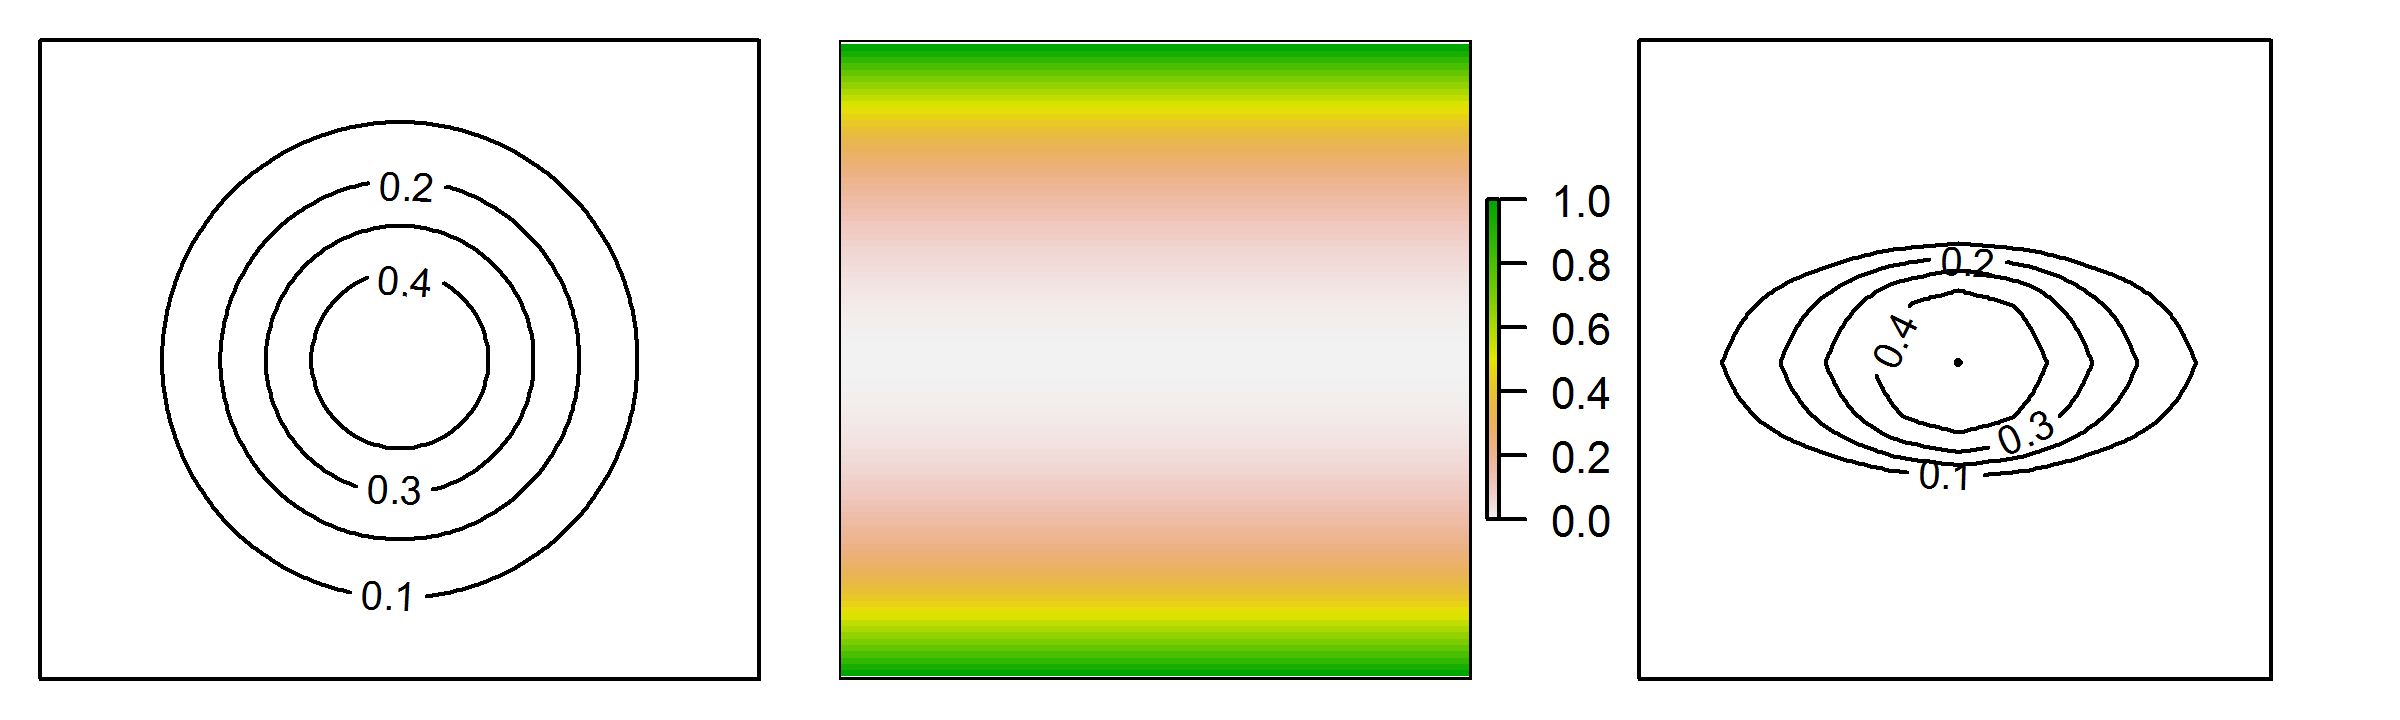
\includegraphics[width=5in,height=1.3in]{Ch10-EcolDist/figs/distort}
\caption{A symmetric home range (left), a habitat variable (center)
  such as representing an elevation gradient,
  and a non-symmetric home range (right) resulting from the cost imposed on
  movement by the habitat variable.}
\label{fig.distort}
\end{figure}


\section{Least-Cost Path Distance}

We adopt a cost-weighted distance metric here which defines the
effective distance between points by accumulating pixel-specific costs
determined using a cost function defined by the user.  The idea of
cost-weighted distance to characterize animal use of landscapes is
widely used in landscape ecology for modeling connectivity, movement
and gene flow \citep{beier_etal:2008}. For reasons of computational
tractability we consider a discrete landscape defined by a raster of
some prescribed resolution. The distance between any two points ${\bf
  x}$ and ${\bf x}'$ can be represented by a sequence of line segments
connecting neighboring pixels, say ${\bf l}_{1},{\bf
  l}_{2},\ldots,{\bf l}_{m}$. Then the cost-weighted distance between
${\bf x}$ and ${\bf x}'$ is
\begin{equation}
 d({\bf x},{\bf x}')
  =  \sum_{i=1}^{m-1} cost({\bf l}_{i},{\bf l}_{i+1})||{\bf l}_{i} - {\bf l}_{i+1}||
\label{eq.costweighted}
\end{equation}
where $cost({\bf l}_{i},{\bf l}_{i+1})$ is the user-defined cost to
move from pixel ${\bf l}_{i}$ to neighboring pixel ${\bf l}_{i+1}$ in
the sequence.  Given the cost of each pixel, it is a simple matter to
compute the cost-weighted distance between any two pixels, along {\it
  any} path, simply by accumulating the incremental costs weighted by
distances.  In the context of spatial capture-recapture models (and,
more generally, landscape connectivity) we are concerned with the {\it
  minimum} cost-weighted distance, or the {\it least-cost path},
between any two points which we will denote by $d_{lcp}$, which is the
sequence ${\cal P} = ({\bf l}_{1},{\bf l}_{2},\ldots,{\bf l}_{m})$
that minimizes the objective function defined by
Eq. \ref{eq.costweighted}. That is,
\begin{equation}
 d_{lcp}({\bf x},{\bf x}')
  =  \min_{{\cal P}} \sum_{i=1}^{m-1} cost({\bf l}_{i},{\bf l}_{i+1})||{\bf l}_{i} - {\bf l}_{i+1}||
\label{eq.lcp}
\end{equation}
The least-cost path distance can be calculated in
 many geographic information systems and other software packages,
including the {\bf R} package \mbox{\tt
  gdistance} \citep{vanetten:2011} which we use below.

The key ecological aspect of least-cost path modeling is the
development
of models for pixel-specific cost.
In this paper we model cost as a function of one or more covariates
defined on every pixel of the according raster. For example, using a
single covariate $z({\bf x})$ we define the cost of moving from some pixel
${\bf x}$ to neighboring pixel ${\bf x}'$ as
\begin{equation}
\log(  cost({\bf x},{\bf x}'))=  \alpha_{2}\left( \frac{z({\bf
      x})+z({\bf x}')}{2}
\right)
\label{ecoldist.eq.cost}
\end{equation}
Thus, if $\alpha_{2} = 0$ then substituting $\mbox{cost}({\bf x},{\bf x}')
=\exp(0) = 1$ into
Eq. \ref{eq.lcp} will produce the ordinary Euclidean distance
between points. Here we assume the covariate $z$ is positive-valued
and constrain $\alpha_{2}\ge 0$ so as to avoid
negative costs. While not necessarily problematic from a mathematical
standpoint, negative costs are unrealistic biologically. 

The use of least-cost path models to model landscape connectivity has
been around for a long time. And, although $\alpha_{2}$ is rarely
known, conservation biologists design linkages that require this
resistance value as input \citep[see][and articles cited
therein]{beier_etal:2008}.  However, formal inference (e.g.,
estimation) of parameters is not often done.  Instead, in many
existing applications of least-cost path analysis, the parameter
$\alpha_{2}$ is fixed by the investigator, or based on expert opinion
\citep{beier_etal:2008}, although recently researchers have begun to
define costs based on resource selection functions, animal movement
\citep{tracy:2006, fortin_etal:2005}, or genetic distance data (e.g.,
\citet{gerlach_musolf:2000}; \citet{epps_etal:2007};
\citet{schwartz_etal:2009}. We address the integration of resource
selection models based on telemetry data with SCR models in
Chapt. \ref{chapt.rsf}.


To formalize the use of cost-weighted distance in SCR models, we 
substitute Eq. \ref{eq.lcp} in the expression for encounter
probability (Eq. \ref{eq.encounter}) and maximize the resulting
likelihood which we address below. In doing so, we can directly 
estimate parameters of the least-cost path model, evaluate how 
landscape covariate influence connectivity, and test explicit hypotheses
about these things using only individual level encounter history data
from capture-recapture studies.


\subsection{Example of Computing Cost-weighted distance}


{\bf XXXX Kimmy: Reconcile the raster example here with what is in the
  Appendix of the accepted Ecology paper. XXXXX}

As an example of the cost-weighted distance calculation consider the
following landscape comprised of 16 pixels with unit spacing
identified as follows, along with the pixel-specific cost:
\begin{center}
\begin{verbatim}
         pixel ID                Cost
       1  5  9  13          100   1   1  1
       2  6 10  14          100 100   1  1
       3  7 11  15          100 100 100  1
       4  8 12  16          100 100   1  1
\end{verbatim}
\end{center}
This simple cost raster is shown in Fig. \ref{ecoldist.fig.raster}. We
assume the scale is such that the distance between neighboring pixels
in any cardinal direction is 1 unit, and the distance between
neighbors on a diagonal is $\sqrt{2}$ units.  We assigned low cost of
1 to ``good habitat'' pixels (or pixels we think of as ``highly
connected'' by virtue of being in good habitat) and, conversely, we
assign high cost (100) to ``bad habitat''. So the shortest
cost-weighted distance between pixels 5 and 9 in this example is just
1 unit, the shortest cost-distance between pixels 5 and 10 is
$\sqrt{2}(1+1)/2 = 1.414214$ units, the shortest distance between
pixels 4 and 8 is 100 units, while the shortest cost-distance between
4 and 12 is 150.5. A tough one is: what is the shortest distance
between 7 and 16? An individual at pixel 7 can move diagonal (which
has distance $\sqrt{2}$) and pay $sqrt(2)*(100+1)/2 + 1 =72.41778$.

\begin{figure}[h]
\begin{center}
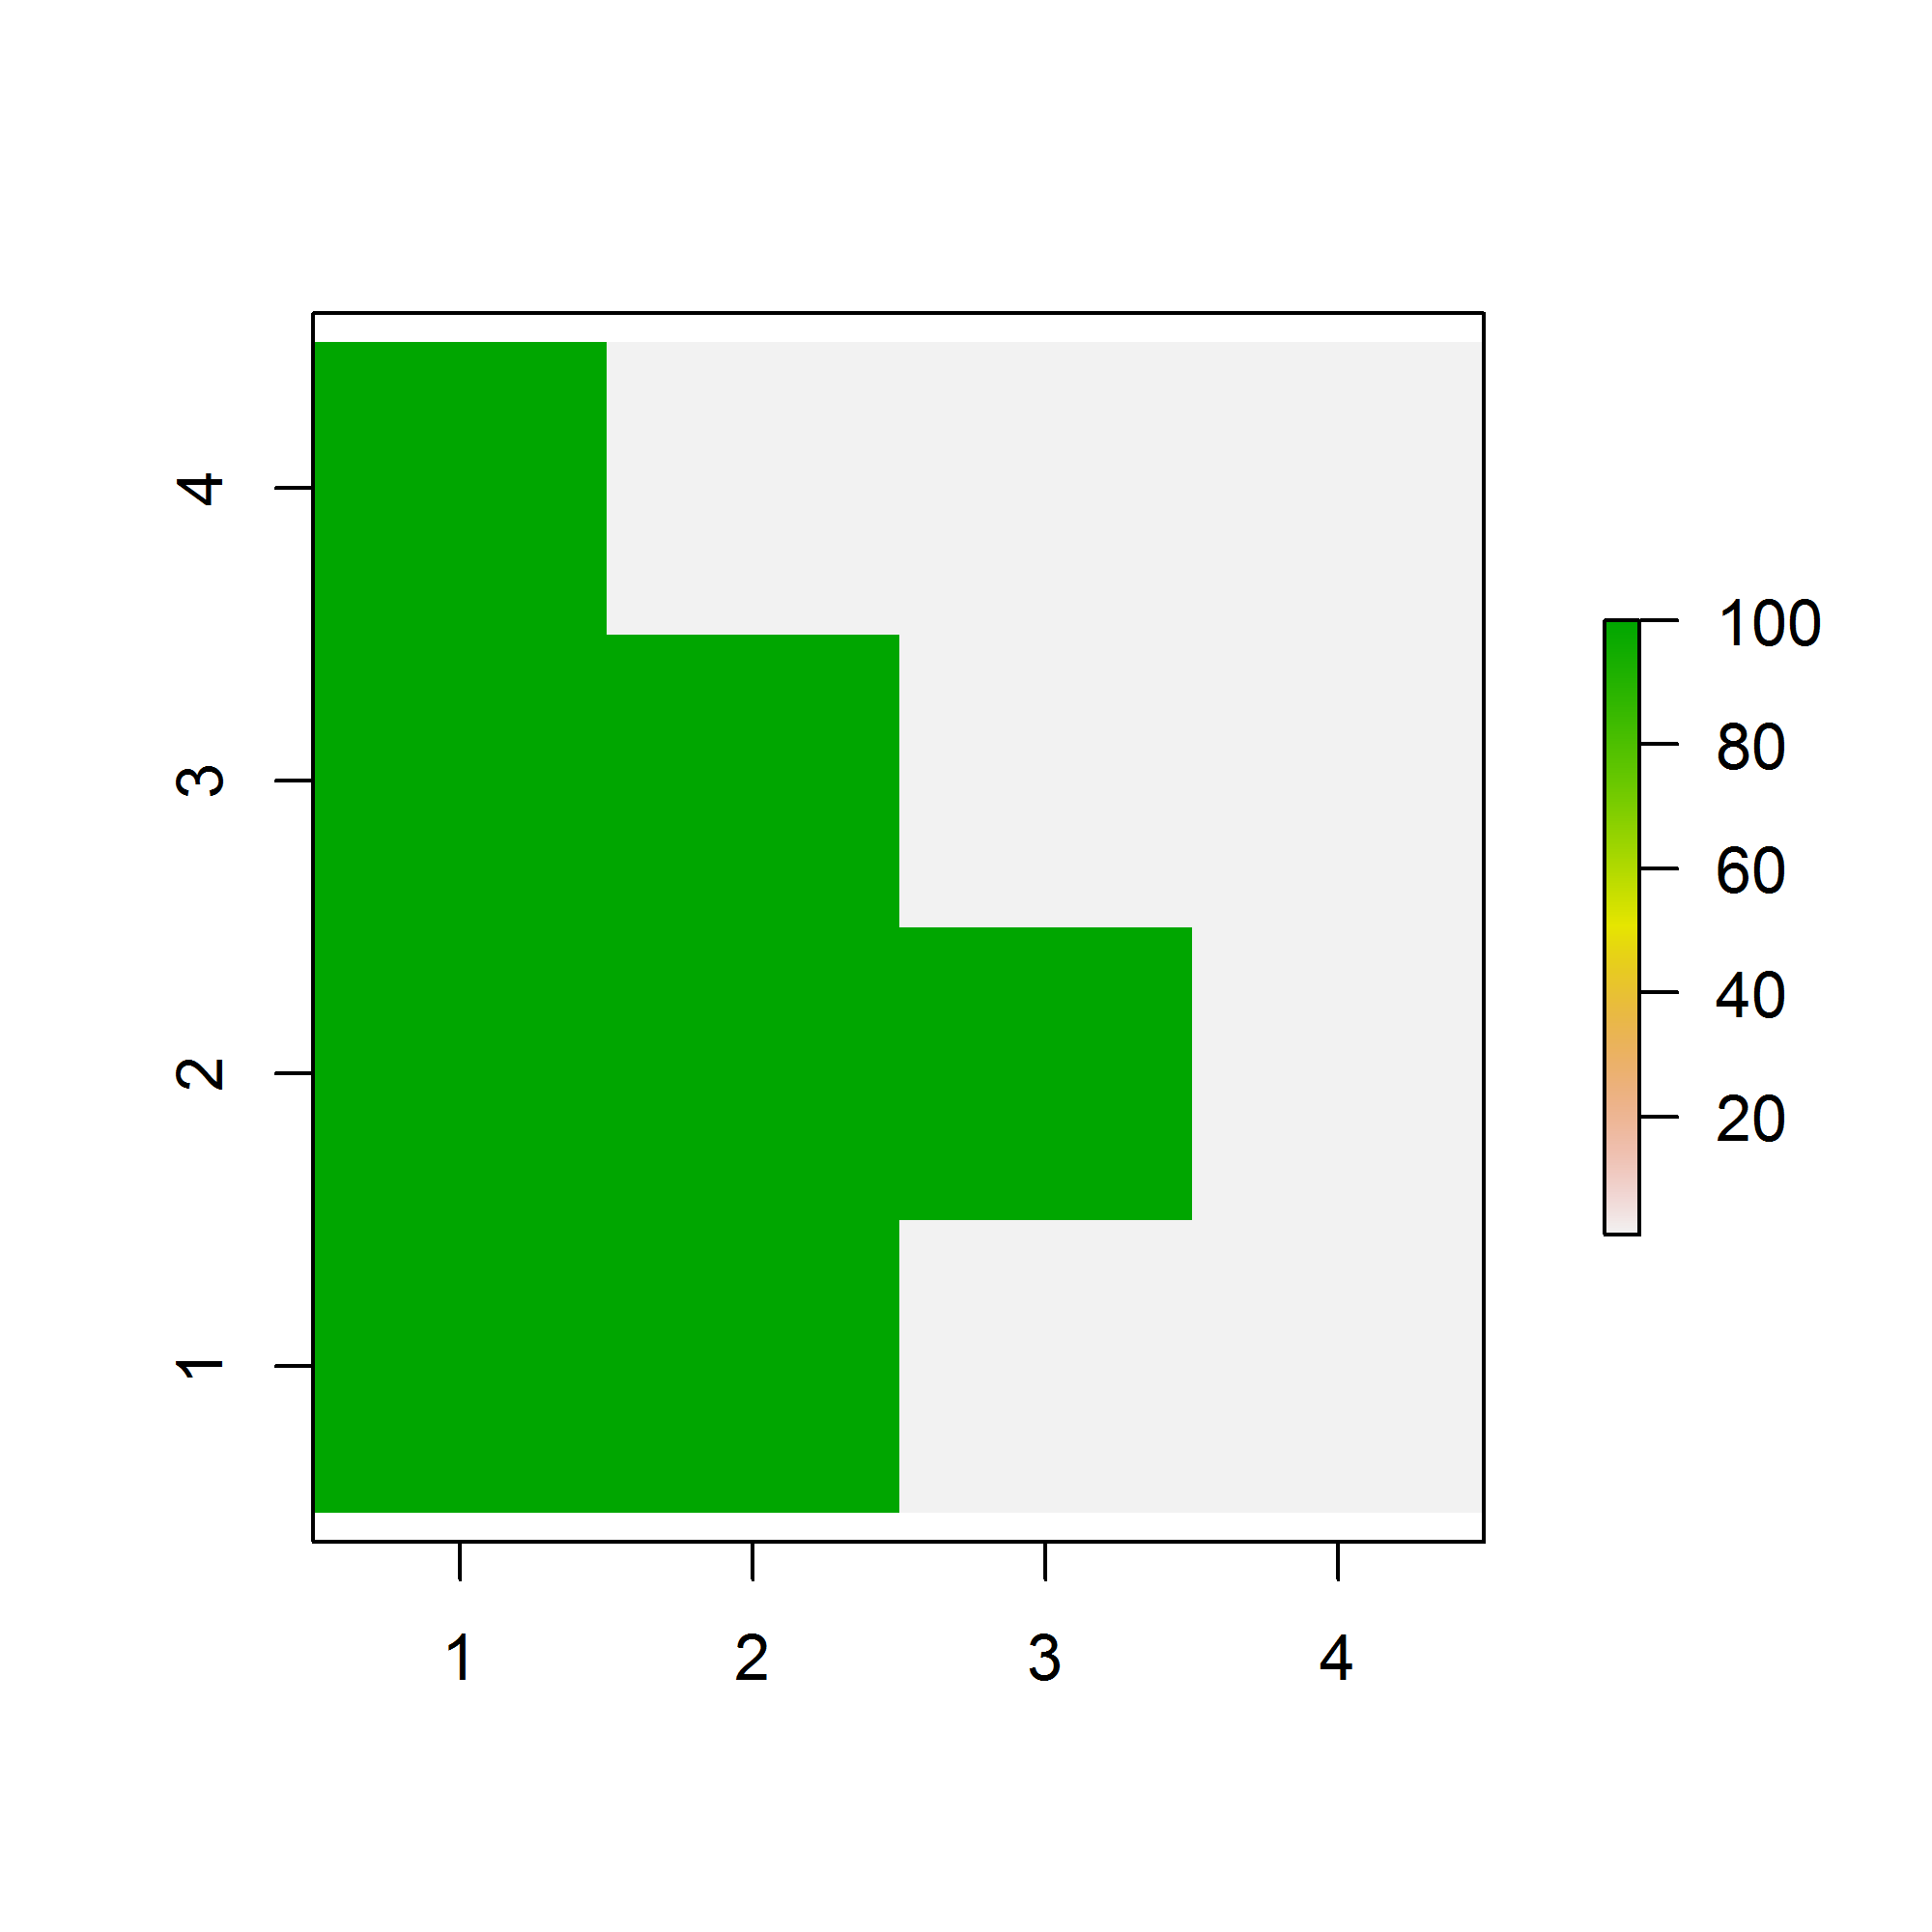
\includegraphics[height=3.25in,width=3.25in]{Ch10-EcolDist/figs/raster_2values}
\end{center}
\caption{A $4 \times 4$ raster depicting a binary cost surface, with cost = 1 (white) or 100 (shaded) to represent ease of movement across a pixel.}
\label{ecoldist.fig.raster}
\end{figure}

Once the cost raster is created, the least-cost path distances are
computed with just a couple {\bf R} commands, and those can be
inserted directly into the likelihood construction for an ordinary
spatial capture-recapture model The {\bf R} package
\mbox{\tt gdistance} calculates least-cost path using  Dijkstra's algorithm
\citep{dijkstra:1959} (from the \mbox{\tt igraph} package
\citep{csardi:2010}).  Using \mbox{\tt gdistance}, we 
define the incremental cost of moving from one pixel to another as the
distance-weighted {\it average} of the 2 pixel costs. We demonstrate
how to do this subsequently.

{\bf Kimmy: Make sure the structure of this example is copied directly
from the Ecology paper that was accepted. There are some things
slightly
different.}

The {\bf R} commands for computing the least-cost distance between all pairs of pixels
are as follows:
\begin{verbatim}
r<-raster(nrows=4,ncols=4)
projection(r)<- "+proj=utm +zone=12 +datum=WGS84"
extent(r)<-c(.5,4.5,.5,4.5)
costs1<- c(100,100,100,100,1,100,100,100,1,1,100,1,1,1,1,1)
values(r)<-matrix(costs1,4,4,byrow=FALSE)
par(mfrow=c(1,1))
plot(r)
\end{verbatim}
Then we use the functions \mbox{\tt transition}, \mbox{\tt
  geoCorrection} {\bf XXX Kimmy do we need this function? XXXX}
 (which is only necessary if the data are not
projected or if cells are considered to have more than 4 neighbors)
 and \mbox{\tt costDistance} to compute the distance
matrix. The transition function computes the cost of making a
transition between
any two pixels, and it operates on the inverse-scale (''conductance'')
and so the
\mbox{\tt transitionFunction} argument is given as $1/mean(x)$.
To compute the cost distance we prescribe a set of points, or  we
can compute it  between
two sets of points (which is handy when one of the sets is of trap
locations, and the other is of individual activity centers).
To compute the distances for pixels in a raster,
we use the center points of each raster.  The {\bf R}
 commands altogether are as follows:
{\small
\begin{verbatim}
tr1<-transition(r,transitionFunction=function(x) 1/mean(x),directions=8)
tr1CorrC<-geoCorrection(tr1,type="c",multpl=FALSE,scl=FALSE)
pts<-cbind( sort(rep(1:4,4)),rep(4:1,4))
costs1<-costDistance(tr1CorrC,pts)
outD<-as.matrix(costs1)
\end{verbatim}
}
Now we can look at the result and see if it makes sense to us. Here we
produce the first 5 columns of this distance matrix to illustrate a
couple of examples of calculating the minimum cost-weighted distance
between points: {\bf XXXX Kimmy: All of these numbers are probably
  different
in the paper's appendix and we need to change them here XXXXX}
\begin{center}
{\small
\begin{verbatim}
> outD[1:5,1:5]
         1         2        3        4         5
1   0.0000 100.00000 200.0000 205.2426  50.50000
2 100.0000   0.00000 100.0000 200.0000  71.41778
3 200.0000 100.00000   0.0000 100.0000 171.41778
4 205.2426 200.00000 100.0000   0.0000 154.74264
5  50.5000  71.41778 171.4178 154.7426   0.00000
\end{verbatim}
}
\end{center}
An interesting case is that between point 1 and 4. Note that simply
taking the shortest Euclidean distance, weighted by cost, produces a
cost-weighted distance of $100 \times 1$ to move from pixel 1 to pixel
2, and similarly from 2 to 3 and 3 to 4, producing a total
cost-weighted distance of $300$. However, the actual {\it least-cost
  path} has cost-weighted distance $205.2426$ which 
 has an individual moving from pixel 1 to 5, then 5
to 10, 10 to 15, 15 to 12, 12 to 8 and 8 to 4, adding up to a cost
weighted distance of 
$205.2426$.


\section{Simulating SCR Data using Ecological Distance}
\label{ecoldist.sec.simulating}

\citet{royle_etal:2012ecol} simulated data based on two hypothetical
landscapes typical of how
cost-weighted distance models might be used in real capture-recapture
problems.  They defined a $20 \times 20$ pixel covariate raster with
extent = $[0.5, 4.5] \times [0.5, 4.5]$ which we imagine to be a 
 coarse landscape covariate, with pixels
having some arbitrary scaling. For example, think of each pixel as
representing, say, a $1 \times 1$ km grid cell in which case 
the raster defines a landscape of $20 \times 20$ km. We suppose
that 16 camera traps are established at the integer coordinates
$(1,1), (1,2), \ldots, (4,4)$. We could think of this as a landscape
within which we're studying a population of ocelots, lynx or some
other cat.

For our analyses here, we characterize cost by one covariate, 
and we consider two specific cases. First is an increasing trend from
the NW to the SE (''systematic covariate''), where $z({\bf x})$ is defined as
$z({\bf x}) = r({\bf x}) + c({\bf x})$ and $r({\bf x})$ and $c({\bf x})$ are just the row and
column, respectively, of the raster.  This might mimic something
related to distance from an urban area or a gradient in habitat
quality due to land use, or environmental conditions such as
temperature or precipitation gradients.  In the second case we make up
a covariate by generating a field of spatially correlated noise to
emulate a typical patchy habitat covariate (``patchy covariate'') such as
tree or understory density. The two covariates are shown in
Fig. \ref{ecoldist.fig.raster100}, along with a sample realization of
$N=100$ individuals (left panel only).  For both covariates we use a
cost function in which transitions from pixel ${\bf x}$ to ${\bf x}'$
is given by:
\[
 log(cost({\bf x},{\bf x}'))=  \alpha_2 \frac{z({\bf x}) + z({\bf x}')}{2}
\]
where $\alpha_2 = 1$ for simulating the observed data.
 Remember that with $\alpha_2=0$ the
model reduces to one in which the cost of moving across each pixel is
constant, and therefore Euclidean distance is operative.

\begin{figure}[h]
\begin{tabular}{ll}
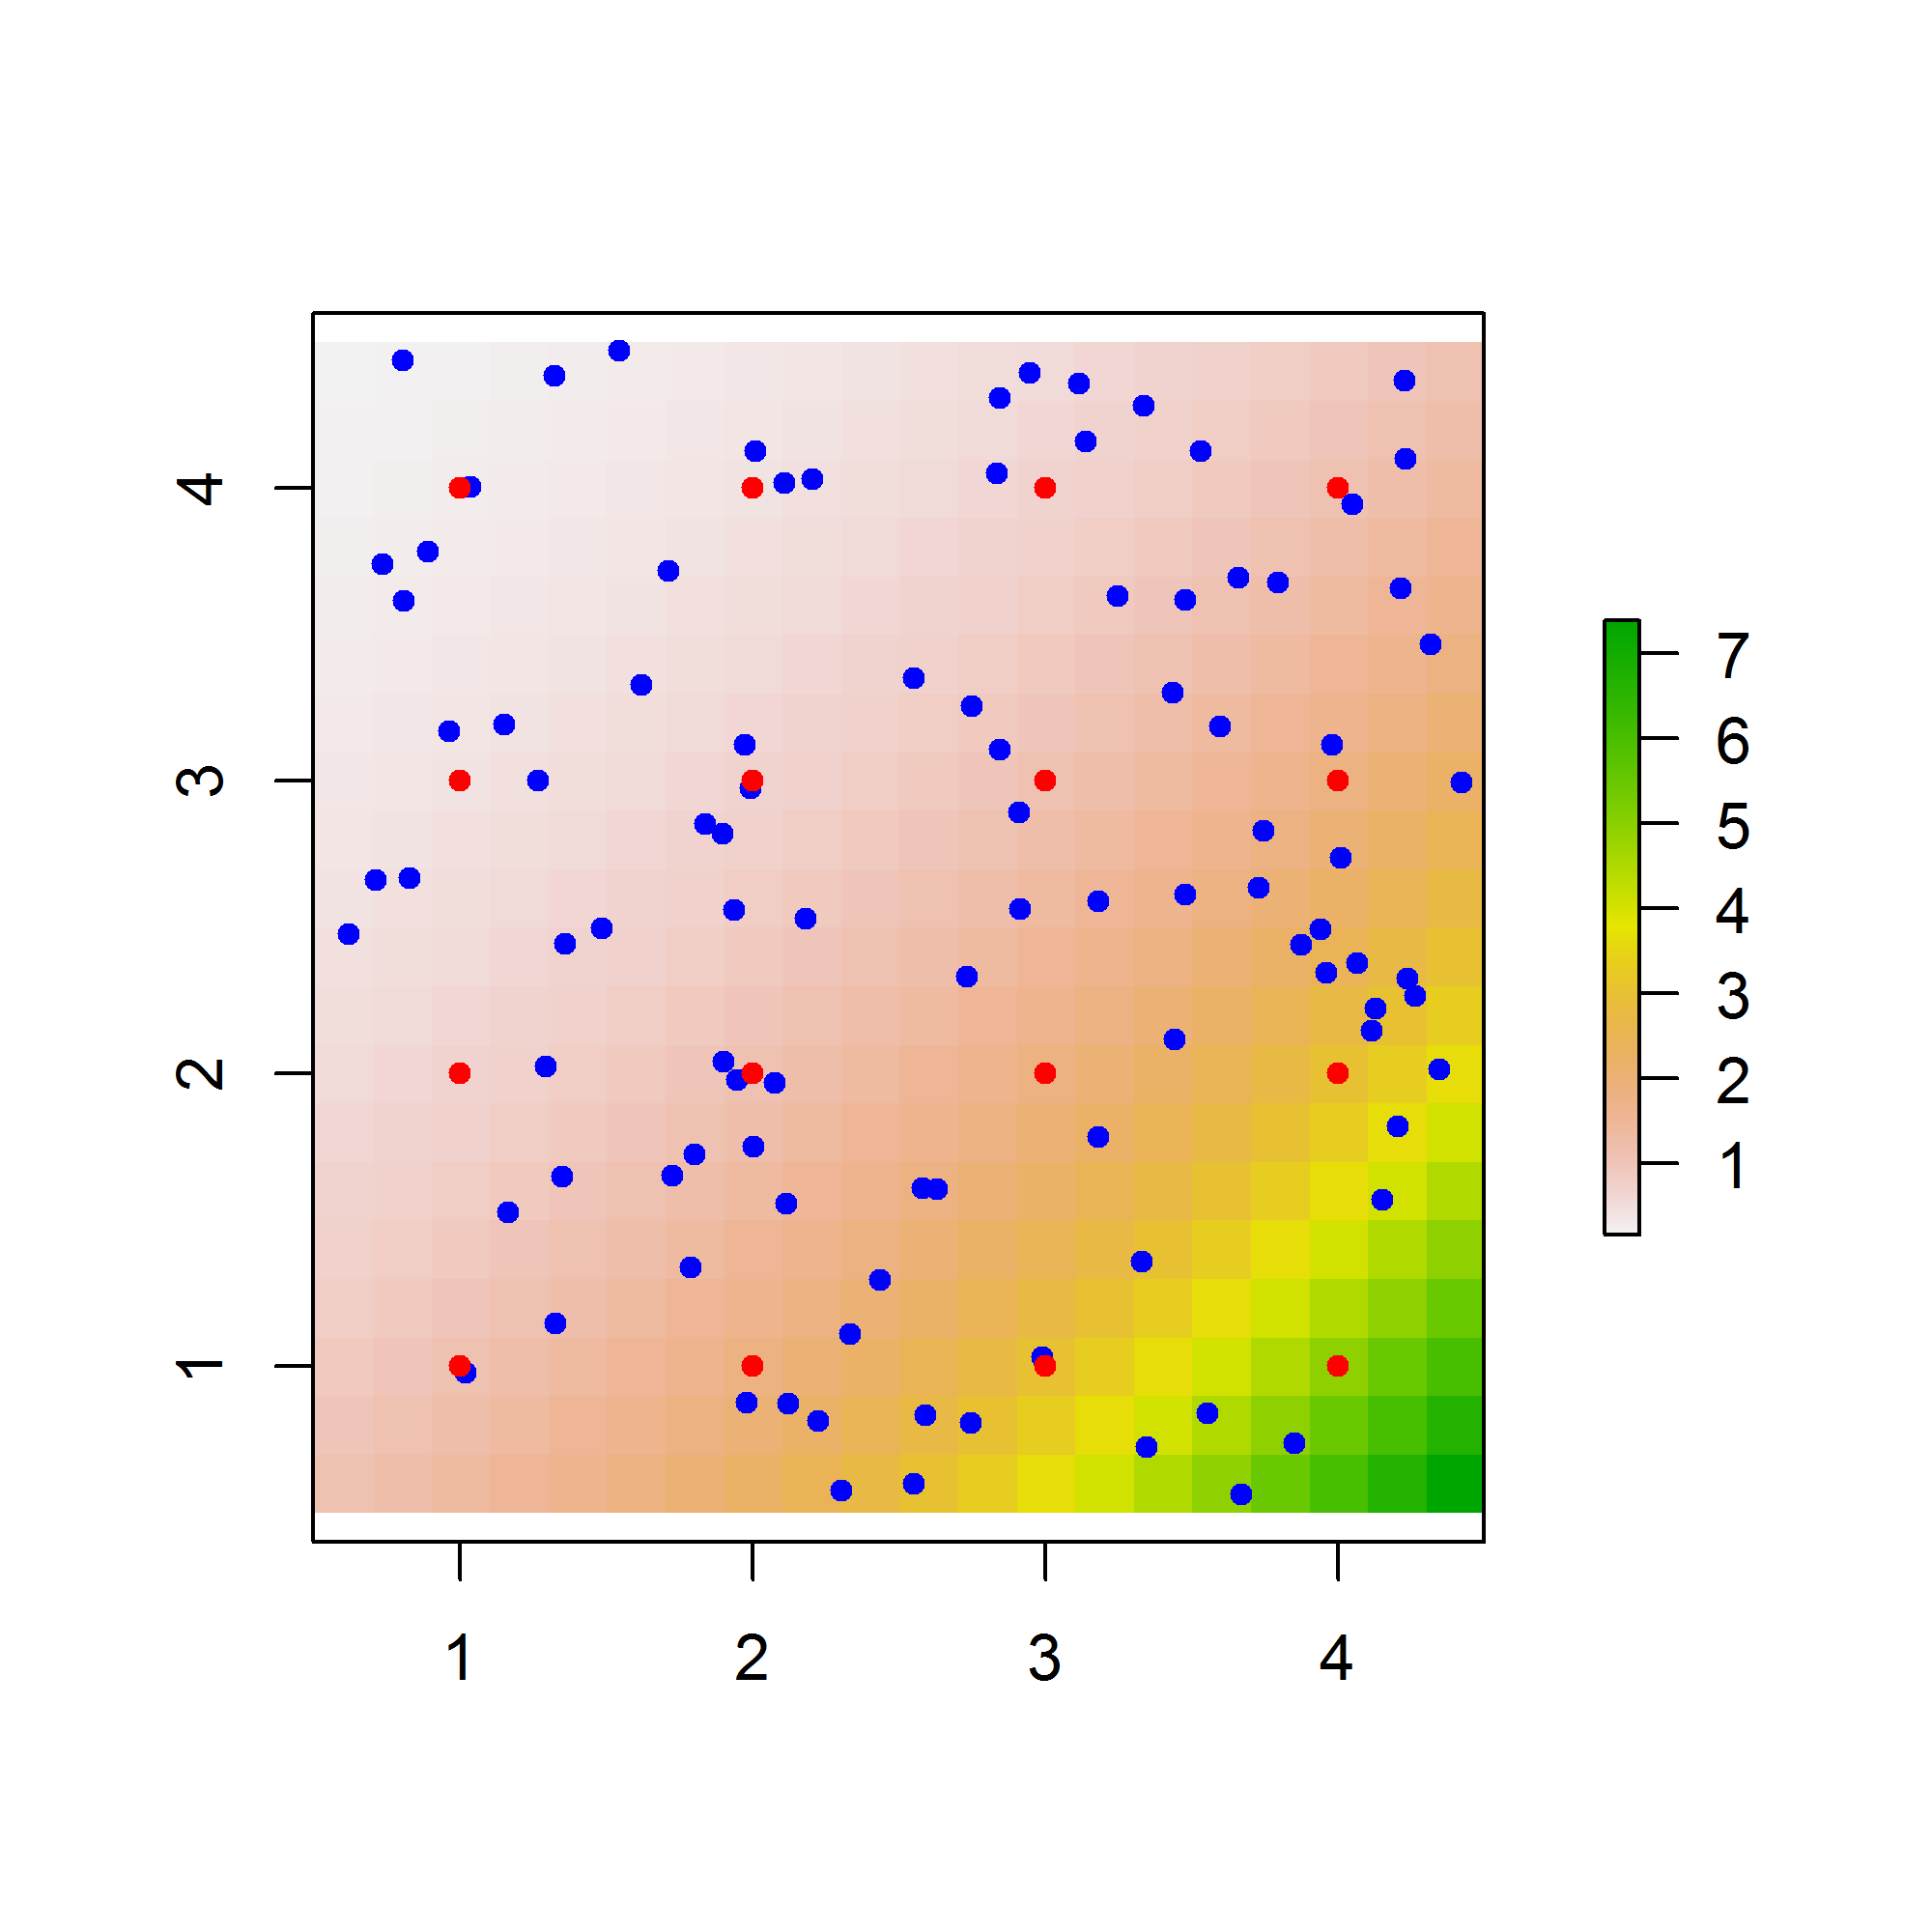
\includegraphics[height=2.5in,width=2.5in]{Ch10-EcolDist/figs/raster_withN100}
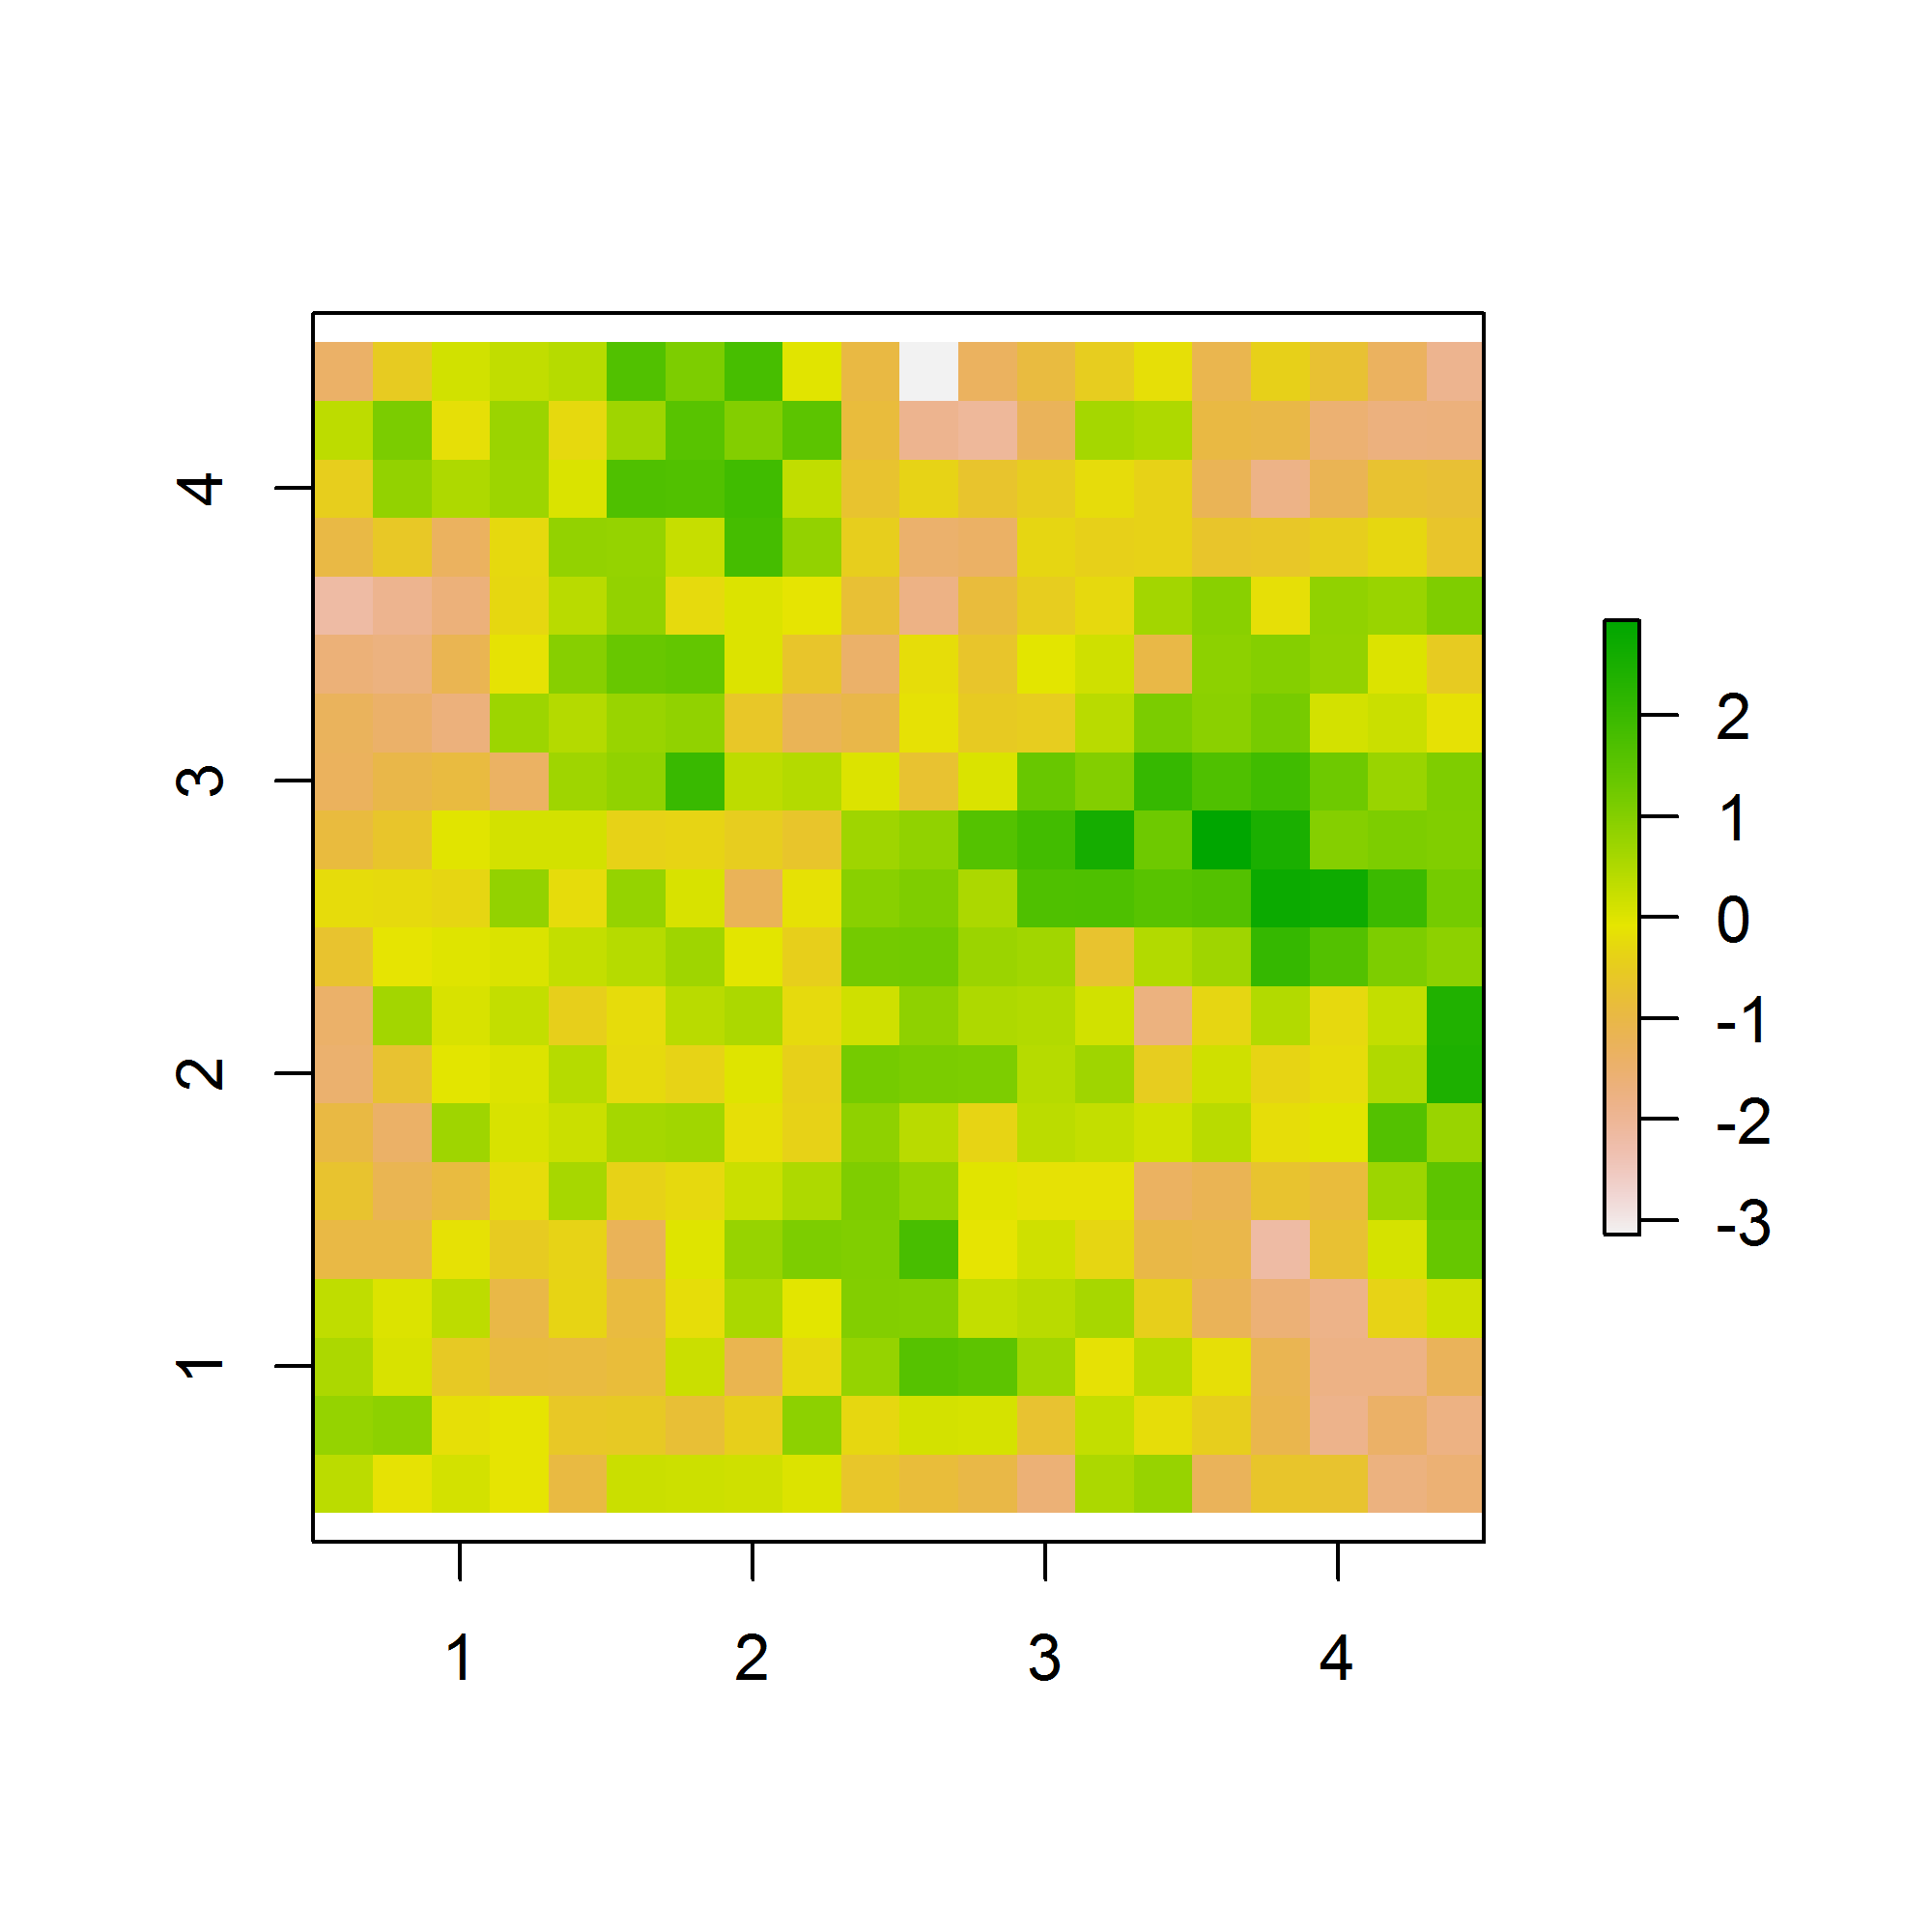
\includegraphics[height=2.5in,width=2.5in]{Ch10-EcolDist/figs/raster_krige} &
\end{tabular}
\caption{Two covariates (defined on a $20 \times 20$ grid) used in simulations.
 Left panel shows a 
 covariate with systematic structure meant 
to mimic distance from some feature, and the right panel
 shows a ``patchy'' covariate. 
A hypothetical
  realization of $N=100$ activity centers (blue dots) is superimposed
  on the left figure,
along with 16 trap locations. }
\label{ecoldist.fig.raster100}
\end{figure}


When distance is defined by the cost-weighted distance metric given
by Eq. \ref{eq.lcp} then individual space-usage varies
spatially in response to the landscape covariate(s) used in the
distance metric.  As a consequence, home ranges contours are no longer
circular, as in SCR models based on Euclidean distance.
 For example, using one of the covariates we use in
our simulation study below (Fig. \ref{ecoldist.fig.raster100}, right
panel) with a Gaussian pdf detection function but having distance
metric defined by Eq. \ref{eq.lcp}, produces home ranges such
as those shown in Fig. \ref{fig.homeranges}. 


\begin{figure}
\begin{center}
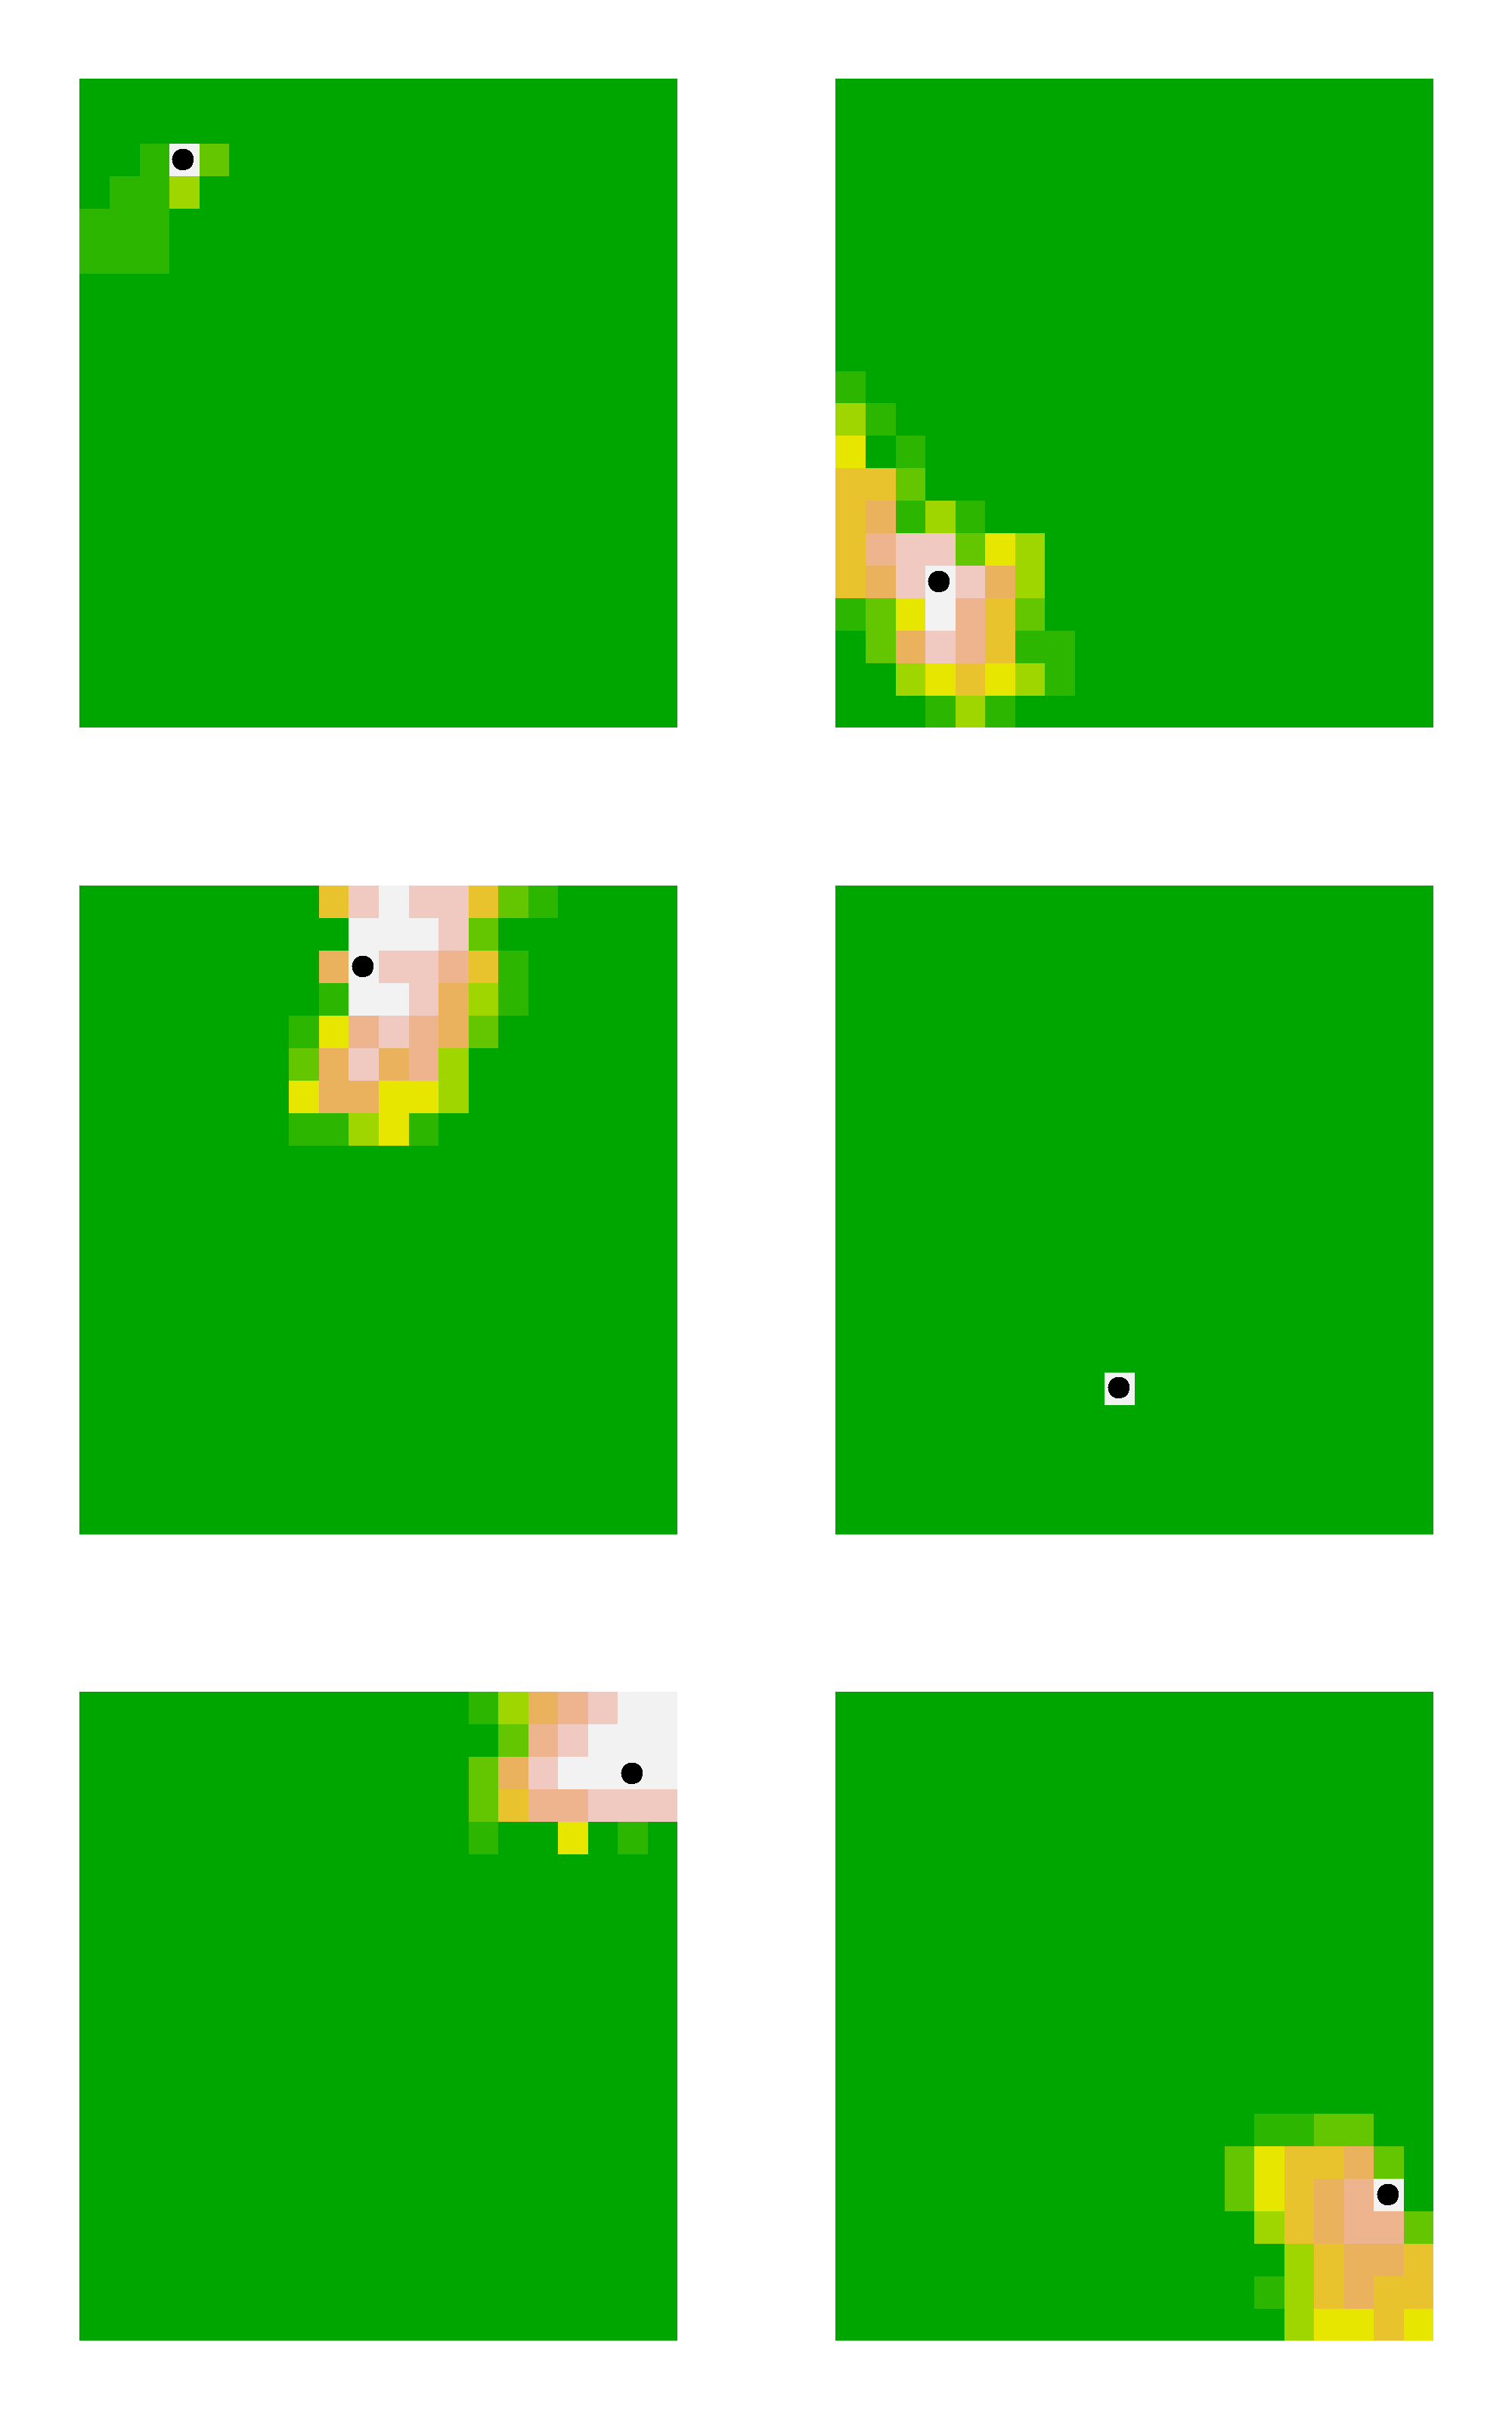
\includegraphics[height=6in,width=3.75in]{Ch10-EcolDist/figs/home_ranges}
\end{center}
\caption{
Typical home ranges for 6 individuals based on the cost surface shown in the right panel of 
  Fig. \ref{ecoldist.fig.raster100} with $\alpha_{2}=1$. The black dot indicates the home
  range center and the pixels around each home range center are shaded
according to the probability of encounter, if a trap were located in
that pixel.
}
\label{fig.homeranges}
\end{figure}

To simulate data, 
 we have to load the \mbox{\tt
scrbook} package and call the function \mbox{\tt make.EDcovariates} to generate
our raster covariates (see the help file for how that is done). We
process the covariate into a least-cost path distance
matrix, and then simulate observed encounter data using standard methods
which we have used many times previously in this book. The complete set
of {\bf R} commands is: {\bf XXXX Kimmy: Test this code! XXXXX}
{\bf XXX Kimmy: Do we need the geocorrection() statement in this code?
  XXXXX}
{\small
\begin{verbatim}
### Grab a covariate
library("scrbook")
out<-make.EDcovariates()
covariate<-out$covariate.patchy
set.seed(2013)

### prescribe some settings
N<-200
alpha0<- -2
sigma<- .5
alpha1<- 1/(2*sigma*sigma)
alpha2<-1
K<- 5
S<-cbind(runif(N,.5,4.5),runif(N,.5,4.5))

# make up some trap locations
xg<-seq(1,4,1); yg<-4:1
traplocs<-cbind( sort(rep(xg,4)),rep(yg,4))
points(traplocs,pch=20,col="red")
ntraps<-nrow(traplocs)

### make a raster and fill it up with the "cost"
r<-raster(nrows=20,ncols=20)
projection(r)<- "+proj=utm +zone=12 +datum=WGS84"
extent(r)<-c(.5,4.5,.5,4.5)
cost<- exp(alpha2*covariate)

### compute least-cost path distance
tr1<-transition(cost,transitionFunction=function(x) 1/mean(x),directions=8)
tr1CorrC<-geoCorrection(tr1,type="c",multpl=FALSE,scl=FALSE)
D<-costDistance(tr1CorrC,S,traplocs)
probcap<-plogis(alpha0)*exp(-alpha1*D*D)

# now generate the encounters of every individual in every trap
# discard uncaptured individuals
Y<-matrix(NA,nrow=N,ncol=ntraps)
for(i in 1:nrow(Y)){
 Y[i,]<-rbinom(ntraps,K,probcap[i,])
}
Y<-Y[apply(Y,1,sum)>0,]
\end{verbatim}
}










\section{Likelihood Analysis of Ecological Distance Models}
\label{ecoldist.sec.mle}

Throughout much of this book we rely on Bayesian analysis by MCMC
mostly using {\bf BUGS}, but sometimes (as in Chapt. \ref{chapt.mcmc})
developing our own implementations. However, occasionally we prefer to
use likelihood estimation, such as when we can compare a set of models
directly by likelihood either to do a direct hypothesis test of a
parameter, or to tabulate a bunch of AIC values. For the class of
models that use least-cost path, we also prefer likelihood methods not
because they have any conceptual or methodological benefit, but simply
because they are more computationally efficient to implement
\citep{royle_etal:2012ecol}.

There are no technical considerations in adapting our formulation of
maximum likelihood estimation \citep{borchers_efford:2008} from
Chapt. \ref{chapt.mle} for the class of models based on least-cost
path (see the appendix in \citet{royle_etal:2012ecol} for complete details).
Likelihood analysis is really just a straightforward adaptation in which we
replace the Euclidean distance with least-cost path.  Consider the
Bernoulli model in which the individual- and trap-specific
observations have a binomial distribution conditional on the latent
variable ${\bf s}_{i}$:
\begin{equation}
  y_{ij}| {\bf s}_{i} \sim \mbox{Binomial}(K, p_{\bm \alpha}(d_{lcp}({\bf x}_{j},{\bf s}_{i};\alpha_{2}); \alpha_{0}, \alpha_{1})
\label{ecoldist.eq.cond-on-s}
\end{equation}
where we have indicated the dependence of $p$ on the parameters
${\bm \alpha} =(\alpha_{0},\alpha_{1},\alpha_{2})$, and also $d_{lcp}$ which
itself depends on $\alpha_{2}$, and the latent variable ${\bf s}$.
We note that the only difference between likelihood analysis of this
model and the standard Bernoulli model, is the use of $d_{lcp}$ here. 


XXXXX Andy here XXXXXXXXXXXXXXXXXXXX

For the random effect we have ${\bf s}_{i} \sim  \mbox{Uniform}({\cal
  S})$, we can easily compute the integrated likelihood.

We have an R script in the \mbox{\tt scrbook} package?
adapated from Royle et al. .... XXXXXXXX

We provide an {\bf R} function to evaluate the likelihood, and
optimize it 
using the {\bf R} function \mbox{\tt nlm}.
The likelihood is given in the {\tt scrbook} package as the function
\mbox{\tt intlik3ed}. The help file
provides an example of its usage and for simulating data.
To use this function the cost covariate $z({\bf x})$ has to be of class
\mbox{\tt RasterLayer} which requires packages \mbox{\tt sp} and
\mbox{\tt raster} to manipulate.
%The following is a stylized and more concise version of the actual
%function, and 
%We apply this in the following section.


\begin{comment}
{\small
\begin{verbatim} 
intlik3ed<-function(start=NULL,y=y,K=NULL,X=traplocs, distmet="ecol",
                    covariate,alpha2=NA){

### The covariate is a raster, here we extract needed attributes
nc<-covariate@ncols
nr<-covariate@nrows
Xl<-covariate@extent@xmin
Xu<-covariate@extent@xmax
Yl<-covariate@extent@ymin
Yu<-covariate@extent@ymax

### compute the integration grid
delta<- (Xu-Xl)/nc
xg<-seq(Xl+delta/2,Xu-delta/2,delta)
yg<-seq(Yl+delta/2,Yu-delta/2,delta)
npix.x<-length(xg)
npix.y<-length(yg)
G<-cbind(rep(xg,npix.y),sort(rep(yg,npix.x)))
nG<-nrow(G)

## compute distance matrix
if(distmet=="euclid")
D<- e2dist(X,G)

if(distmet=="ecol"){
if(is.na(alpha2))
alpha2<-exp(start[4])
cost<- exp(alpha2*covariate)
tr1<-transition(cost,transitionFunction=function(x) 1/mean(x),directions=8)
tr1CorrC<-geoCorrection(tr1,type="c",multpl=FALSE,scl=FALSE)
D<-costDistance(tr1CorrC,X,G)
}

alpha0<-start[1]; alpha1<-start[2]; n0<-exp(start[3])

probcap<- (exp(alpha0)/(1+exp(alpha0)))*exp(-alpha1*D*D)
Pm<-matrix(NA,nrow=nrow(probcap),ncol=ncol(probcap))
ymat<-rbind(y,rep(0,ncol(y)))
lik.marg<-rep(NA,nrow(ymat))
for(i in 1:nrow(ymat)){
Pm[1:length(Pm)]<- (dbinom(rep(ymat[i,],nG),rep(K,nG),probcap[1:length(Pm)],log=TRUE))
lik.cond<- exp(colSums(Pm))
lik.marg[i]<- sum( lik.cond*(1/nG) )
}
nv<-c(rep(1,length(lik.marg)-1),n0)
part1<- lgamma(nrow(y)+n0+1) - lgamma(n0+1)
part2<- sum(nv*log(lik.marg))
out<-  -1*(part1+ part2)
out
}
\end{verbatim}
}
\end{comment}


\subsection{Example of SCR with Least-Cost Path}

Now we use the {\bf R} function \mbox{\tt nlm} along with
our \mbox{\tt intlik3ed} function to  obtain the MLEs of the
model parameters for the data simulated 
in sec. \ref{ecoldist.sec.simulating}.
 We'll do that for both the standard Euclidean distance
and then for the ecological distance based on the ``patchy''
covariate using the following commands:
{\small
 \begin{verbatim}
frog1<-nlm(intlik3ed,c(alpha0,alpha1,3)),hessian=TRUE,y=Y,K=K,X=traplocs,
               distmet="euclid",covariate=covariate,alpha2=1)

frog2<-nlm(intlik3ed,c(alpha0,alpha1,3,-.3),hessian=TRUE,y=Y,K=K,X=traplocs,
               distmet="ecol",covariate=covariate,alpha2=NA)
\end{verbatim}
}

The abbreviated output for the two model fits is shown in Table XXX.
{\bf XXXXXX KIMMY: Put this in a table like the one later in this chapter XXXXXX}
\begin{verbatim}
Distance     -LL         alpha0     alpha1      log(n0)      alpha2
true value                -2         2          [??]           1
euclidean   133.4951  -1.885005    1.247305    3.549064      --
LCP (truth)  70.11916 -1.78029983  2.47083431  4.45867628  0.04560194
\end{verbatim}



The model based on least-cost path (the data generating model) appears
to be much preferred in terms of negative log-likelihood.
The output parameter order is $(\alpha_{0}, \alpha_{1}, log(n_{0}), and
log(\alpha_{2}))$ (remember, we want to keep $\alpha_{2}$
positive, so it's logarithm is estimated). 
The data generating parameter values were
$\alpha_{0} = - 2$, 
$\alpha_{1} = 2$ and $log(\alpha_{2}) = 0$.
The simulated sampling produced a sample of 96 individuals and so
$n_{0} = 104$, so $log(n_{0}) = 4.64$. We see that the 
 MLEs of the least-cost path model are pretty close whereas they are
 not so close under the misspecified model based on Euclidean distance.






\section{Bayesian Analysis}

While implementation of these ecological distance SCR models is
reasonably straightforward, we do not believe the model can be fitted
in the  {\bf BUGS} engines because least-cost path distance cannot be computed.
It would be possible to fit the models
in {\bf BUGS} if the parameter $\alpha_{2}$ was fixed. In that case,
one could compute the distance matrix ahead of time and reference the
required elements for a given ${\bf s}$.
Alternatively, it would be possible to write a custom MCMC routine
using the methods we present in Chapt. \ref{chapt.mcmc}, although we
have not yet developed our own MCMC implementation of SCR models with
ecological distance metrics. 


\section{Simulation Evaluation of the MLE}

\citet{royle_etal:2012ecol}
carried-out a limited simulation study to evaluate the
general statistical performance of the density estimator under
this new model, the effect of mis-specifying the model with a
normal Euclidean distance metric and evaluate the general bias and
precision properties of the MLE.
We recapitulate their results here.
For population sizes of 100 and 200, individuals with activity
centers randomly distributed on the $20 \times 20$ landscape, they
subjected individuals
to encounter by 16 traps arranged in a $4\times 4$ grid
using a Gaussian
encounter model with least-cost path distance metric:
\[
\log(p_{ij})= \alpha_{0} + \alpha_{1} d_{lcp}({\bf x}_{j},{\bf
  s}_{i}; \alpha_{2})^{2}
\]
where  $\alpha_{0} = -2$ and $\alpha_{1} = 2$, the latter value
corresponding to $\sigma = 0.5$ of a stationary bivariate normal home
range model.  Different numbers of replicate samples were considered,
$K=3,5,10$
(e.g., nights in a camera trapping study), in order
to produce varying sample
sizes.
For each of the ``systematic'' and ``patchy'' landscapes defined
previously, 200 data sets were simulated and, for each of those, two
different models were fitted: the misspecified Euclidean distance
model; and (ii) the true data-generating model but estimating the
relative cost parameter by maximum likelihood.

\subsection{Simulation Results}

For both landscapes and all simulation conditions (levels of $K$ and
$N$) the average sample sizes of individuals captured are given in
Tab. \ref{tab.samplesize}.  
\begin{table}[h]
\centering
\caption{
Expected sample sizes of captured individuals under each configuration of
$N$ (population size for the prescribed state-space) and $K$ (number of replicate samples).
}
\begin{tabular}{l|rrrr}
 & \multicolumn{2}{c}{Systematic} & \multicolumn{2}{c}{Patchy}  \\
    & N=100 &  N=200  &   N=100 &  N=200  \\ \hline
K=3 &  38.69 &   78.17  &   37.30 &   74.93  \\
K=5 &  51.10 &  103.18  &   51.89 &  103.71 \\
K=10&  65.81 &  132.39  &   69.44 &  138.76 \\
\end{tabular}
\label{tab.samplesize}
\end{table}
The simulation results for estimating $N$
for the prescribed state-space are presented in Tab.
\ref{tab.results1}.  For the ``patchy'' landscape we see extreme
bias in estimates of $N$ when the Euclidean distance is used. There is
moderate small sample bias of 3-5\% in the MLE of $N$ using the
least-cost distance which becomes negligible as $K$ increases. For
$N=200$ the bias is on the order of 2\% for the lowest sample size
case ($K=3$) but negligible otherwise.  Interestingly, for the
landscape exhibiting systematic structure, there is a persistent bias
in the MLE of $N$ of 1-3\% even for the highest level of $K$.
As noted by \citet{royle_etal:2012ecol}, 
this is due to the fact that
the state-space is small relative to the extent of the trapping grid and
sensitivity to a state-space that is too small is expected because the
support of the integrand is truncated. In the particular case of the
systematic landscape, we find that, in the NW corner of the raster
where cost of movement is low, individuals use large areas of space,
and the fitted model is under-stating the apparent
heterogeneity in encounter probability for the prescribed raster.  \citet{royle_etal:2012ecol}
found that the issue is resolved when the traps are moved away from
the boundary (results shown in Tab. \ref{tab.results3}).

The performance of estimating the cost parameter $\alpha_{2}$ mirrors
the results for estimating $N$ for the prescribed state space. In the
patchy landscape where we don't expect a systematic gradient in space
usage around the edge of the state-space, we see
(Table \ref{tab.results2}) that $\alpha_{2}$ is estimated with
diminishing bias as the sample size increases, but with persistent
bias due to truncation of the likelihood under the systematic
landscape which, as with the MLE of $N$, is resolved by moving the
traps away from the edge of the raster. Equivalently, in practice,
this could be resolved by expanding the raster away from the trap
locations so that all regions used by animals exposed to capture are
included in the state-space.




\begin{table}[htp]
\label{tab.results1}
{\small
\caption{Simulation results for estimating population size $N$ for a prescribed state-space with
$N=100$ or $N=200$ and various levels of replication ($K$) chosen to affect the observed sample
size of individuals (Tab. \ref{tab.samplesize}). For each simulated
data set, the SCR model was fitted by maximum likelihood with
standard Euclidean distance (``euclid''), or least-cost path 
(``lcp''), which was the true data-generating model.
The summary statistics of the
sampling distribution reported are the mean, standard deviation
(``SD'') and quantiles (0.025, 0.50, 0.975).
}
{\bf Systematic trend raster:} \\
\begin{tabular}{l|rrrrr|rrrrr}
         & \multicolumn{5}{c}{N=100   } & \multicolumn{5}{c}{N=200  }  \\
         &   mean &  SD  & 0.025 & 0.50 & 0.975  & mean  & SD   & 0.025 & 0.50  & 0.975 \\ \hline
K=3      &        &      &       &      &        &       &      &       &       &       \\
euclid   &   63.65& 12.62& 44.77 & 61.17&  90.98 & 126.68& 17.05&  98.93& 124.49& 168.26 \\
lcp      &  101.93& 21.68& 67.95 &101.56& 156.21 & 201.58& 28.14& 154.96& 200.15& 263.20\\
K=5      &        &      &       &      &        &       &      &       &       &        \\
euclid   &  64.60 & 7.11 & 51.52 & 63.86&  77.33 & 130.02& 10.25& 113.48& 128.96& 151.32\\
lcp      &  98.94 &12.97 & 74.68 & 99.00& 123.88 & 198.80& 19.60& 166.87& 197.97& 239.46\\
K=10     &        &      &       &      &        &       &      &       &       &       \\
euclid   &  69.24 & 4.83 & 59.37 & 69.47&  79.18 & 139.83&  7.62& 125.65& 139.65& 154.82\\
lcp      &  97.53 & 8.18 & 82.02 & 97.62& 113.16 & 195.19& 13.28& 171.63& 194.58& 217.96\\ \hline
\end{tabular}
\\
{\bf Patchy ``random'' raster: } \\
\begin{tabular}{l|rrrrrrrrrr}
         & \multicolumn{5}{c}{N=100  } & \multicolumn{5}{c}{N=200   }  \\
         &   mean &  SD  & 0.025 & 0.50  & 0.975  & mean  & SD   & 0.025 & 0.50  & 0.975 \\ \hline
K=3      &        &      &       &       &        &       &      &       &       &       \\
euclid   &  78.68 & 18.12& 49.40 & 76.34 & 125.47 & 154.34& 33.74& 107.00& 146.34& 221.43\\
lcp      & 110.96 & 28.65& 69.55 &106.98 & 181.84 & 208.77& 49.29& 141.68& 197.89& 325.77\\
K=5      &        &      &       &       &        &       &      &       &       &        \\
euclid   &  77.85 & 11.55& 59.17 & 77.44 & 101.14 & 153.39& 15.57& 129.31& 149.54& 185.38\\
lcp      & 104.44 & 15.79& 78.38 &101.47 & 139.55 & 200.91& 20.78& 164.42& 200.47& 246.46\\
K=10     &        &      &       &       &        &       &      &       &       &       \\
euclid   &  78.01 & 5.26 & 68.00 & 77.96 & 87.81  & 156.27&  8.51& 142.17& 156.05& 174.55\\
lcp      & 100.42 & 7.56 & 86.72 &100.34 & 115.47 & 198.45& 11.44& 180.06& 198.04& 219.52\\ \hline
\end{tabular}
}
\end{table}





\begin{table}[htp]
\centering
\caption{
Mean of sampling distribution of the cost function parameter
$\alpha_{2}$ for the different simulation
conditions.
}
\begin{tabular}{l|rrrr}
 & \multicolumn{2}{c}{Patchy} & \multicolumn{2}{c}{Systematic} \\
    & N=100 &  N=200  &   N=100 &  N=200  \\ \hline
$K=3$  &   1.05&    1.03 &     1.17 & 1.14 \\
$K=5$  &   1.02&    1.01 &     1.12 &1.12 \\
$K=10$ &   1.01&    1.00 &     1.10 &1.08 \\
\end{tabular}
\label{tab.results2}
\end{table}




\begin{table}[htp]
{\tiny
\caption{Simulation results for estimating population size $N$ for a prescribed state-space with
$N=100$ or $N=200$ and various levels of replication ($K$) chosen to affect the observed sample
size of individuals. These results correspond to those of the
systematic landscape in Table XXXXXXX  except with the traps
moved 0.5 units in from the boundary of the landscape.
Each grouping of 2 rows (for a given value of $K$) summarizes the
performance of $\hat{N}$ under models based on 
Euclidean distance  (``euclid'') and 
a model based on least-cost path, which was the true data-generating model.
The summary statistics of the
sampling distribution reported are the mean, standard deviation
(``SD'') and quantiles (0.025, 0.50, 0.975).
}
\begin{tabular}{l|rrrrr|rrrrr}
         & \multicolumn{5}{c}{N=100   } & \multicolumn{5}{c}{N=200  }  \\
         &   mean &  SD  & 0.025 & 0.50 & 0.975  & mean  & SD   & 0.025 & 0.50  & 0.975 \\ \hline
K=3      &        &      &       &      &        &       &      &       &       &       \\
euclid   &   84.48& 20.42& 51.16 & 81.51& 140.62 &163.70 &24.55 &126.64 &157.67 &223.63 \\
lcp      &  105.90& 26.19& 65.95 &103.40& 182.30 &201.34 &29.54 &161.88 &192.36 &268.98\\
K=5      &        &      &       &      &        &       &      &       &       &       \\
euclid   & 81.21  &11.33 &61.35  &79.20 & 98.86  &163.27 &13.06 &140.21 &162.97 &185.94\\
lcp      & 100.84 &13.15 &79.96  &99.51 &119.08  &200.25 &16.53 &168.88 &199.29 &227.39\\
K=10     &        &      &       &      &        &       &      &       &       &       \\
euclid   &  80.10 & 7.81 &66.45  &79.14 &93.33   &158.40 & 9.25 &142.74 &157.86 &173.18\\
lcp      & 100.10 & 9.88 &82.31  &100.91&116.27  &197.52 &13.03 &169.49 &200.68 &217.82\\ \hline
\end{tabular}
}
\label{tab.results3}
\end{table}





\section{Distance In an Irregular Patch}
\label{ecoldist.sec.buffer}

We provide another illustration of how to employ ecological distance
calculations in SCR models. This example is meant to mimic 
a situation where we have something like a hard habitat boundary
such as a habitat corridor or park unit or some other block
of relatively homogeneous good-quality habitat for some species. This
particular system (shown in Fig. \ref{ecoldist.fig.corridor}) could
be habitat surrounded by a suburban wasteland of McDonalds and
Wal-Marts, much less hospitable habitat for most species.  For our
purposes, we suppose that individuals live within the buffered
``f-shaped'' 
region, although we could also imagine the negative of the
situation in which individuals live outside of the region, so that the
polygon represents a barrier (a lake) or bad habitat (an urban area)
or similar.  We describe the steps for creating this landscape
shortly, so that you can use a similar process to generate more
relevant landscapes for your own problems.

In this case we're not going to estimate any parameters of the cost
function (though you could adapt the analyses of the previous sections
to do that) but instead we're going to use ecological
distance ideas only to constrain movement within (or to avoid)
landscape features. Note that, normally, distance ``as the crow
flies'' would not be suitable for irregular habitat patches such as
that shown in Fig. \ref{ecoldist.fig.corridor}.  


\subsection{Basic Geographic Analysis in R}

In practical applications our landscape will contain one more more
polygons which delineate good or bad habitat or other important
characterisetics of the landscape.  These might exist as GIS
shapefiles or merely as a text file with coordinates defining polygon
boundaries. To work with polygons in the context of SCR models we need
to create a raster, overlay the polygon and assign values to each pixel
depending on whether pixels are in the polygon or not, or how far they
are from polygon boundaries. These operations are relatively easy to
do within a GIS system but we need to be able to do them in ${\bf R}$
in order to compute the least-cost paths needed in the likelihood
evaluation. Some additional geographic analyses have been discussed in
secs. \ref{ecoldist.sec.shapefile} and \ref{mcmc.sec.state-space}
where we talked about reading in the shapefile and doing SCR calculations
on that. 

Often we will have GIS shapefiles that define polygons but, here, we 
 create a set of polygons by
buffering and joining some line segments.
In the {\bf R} library \mbox{\tt scrbook}, we provide
 a function \mbox{\tt make.seg} which allows you to make such
 lines segments given a
specific trap region.  To involve \mbox{\tt make.seg} we first
create a plot region and then call \mbox{\tt make.seg} which has a
single argument being the number of points used to define the line
segment. The user will click on the visual display until the required
number of points has been obtained by \mbox{\tt make.sec}. 
In the following set of commands we generate two line
segments, \mbox{\tt l1} consisting of 9 points and \mbox{\tt l2}
consisting of 5 points, and these reside in a geographic region
enclosedd by $[0,10] \times [0,10]$:
{\small
\begin{verbatim}
library("scrbook")
library("sp")
plot(NULL,xlim=c(0,10),ylim=c(0,10))
l1<-make.seg(9)
plot(l1)
l2<-make.seg(5)
plot(l1)
lines(l2)
\end{verbatim}
}

We used this function as above to create a habitat corridor compose of
line segments of class
\mbox{\tt SpatialLines} from the {\bf R} package \mbox{\tt sp}. The 
corridor can be loaded from \mbox{\tt scrbook} by typing the command
\mbox{\tt data("fakecorridor")}.
This data list has 2 line files in it (\mbox{\tt l1} and \mbox{\tt l2}) and a
trap locations file (\mbox{\tt traps}).
We use some functions from the {\bf R} packages \mbox{\tt sp} and
\mbox{\tt rgeos} to join and
buffer (by 0.5 units) the two segments. The commands are as follows
and the result is shown in Fig. \ref{ecoldist.fig.corridor}.

{\bf XXXX Kimmy: check all of this code! XXXXX}

{\small
\begin{verbatim}
data("fakecorridor")
library("sp")
library("rgeos")

buffer<- 0.5
par(mfrow=c(1,1))
aa<-gUnion(l1,l2)
plot(gBuffer(aa,width=buffer),xlim=c(0,10),ylim=c(0,10))
pg<-gBuffer(aa,width=buffer)
pg.coords<- pg@polygons[[1]]@Polygons[[1]]@coords

xg<-seq(0,10,,40)
yg<-seq(10,0,,40)

delta<-mean(diff(xg))
pts<- cbind(sort(rep(xg,40)),rep(yg,40))
points(pts,pch=20,cex=.5)

in.pts<-point.in.polygon(pts[,1],pts[,2],pg.coords[,1],pg.coords[,2])
points(pts[in.pts==1,],pch=20,col="red")
\end{verbatim}
}

\begin{figure}[h]
\begin{center}
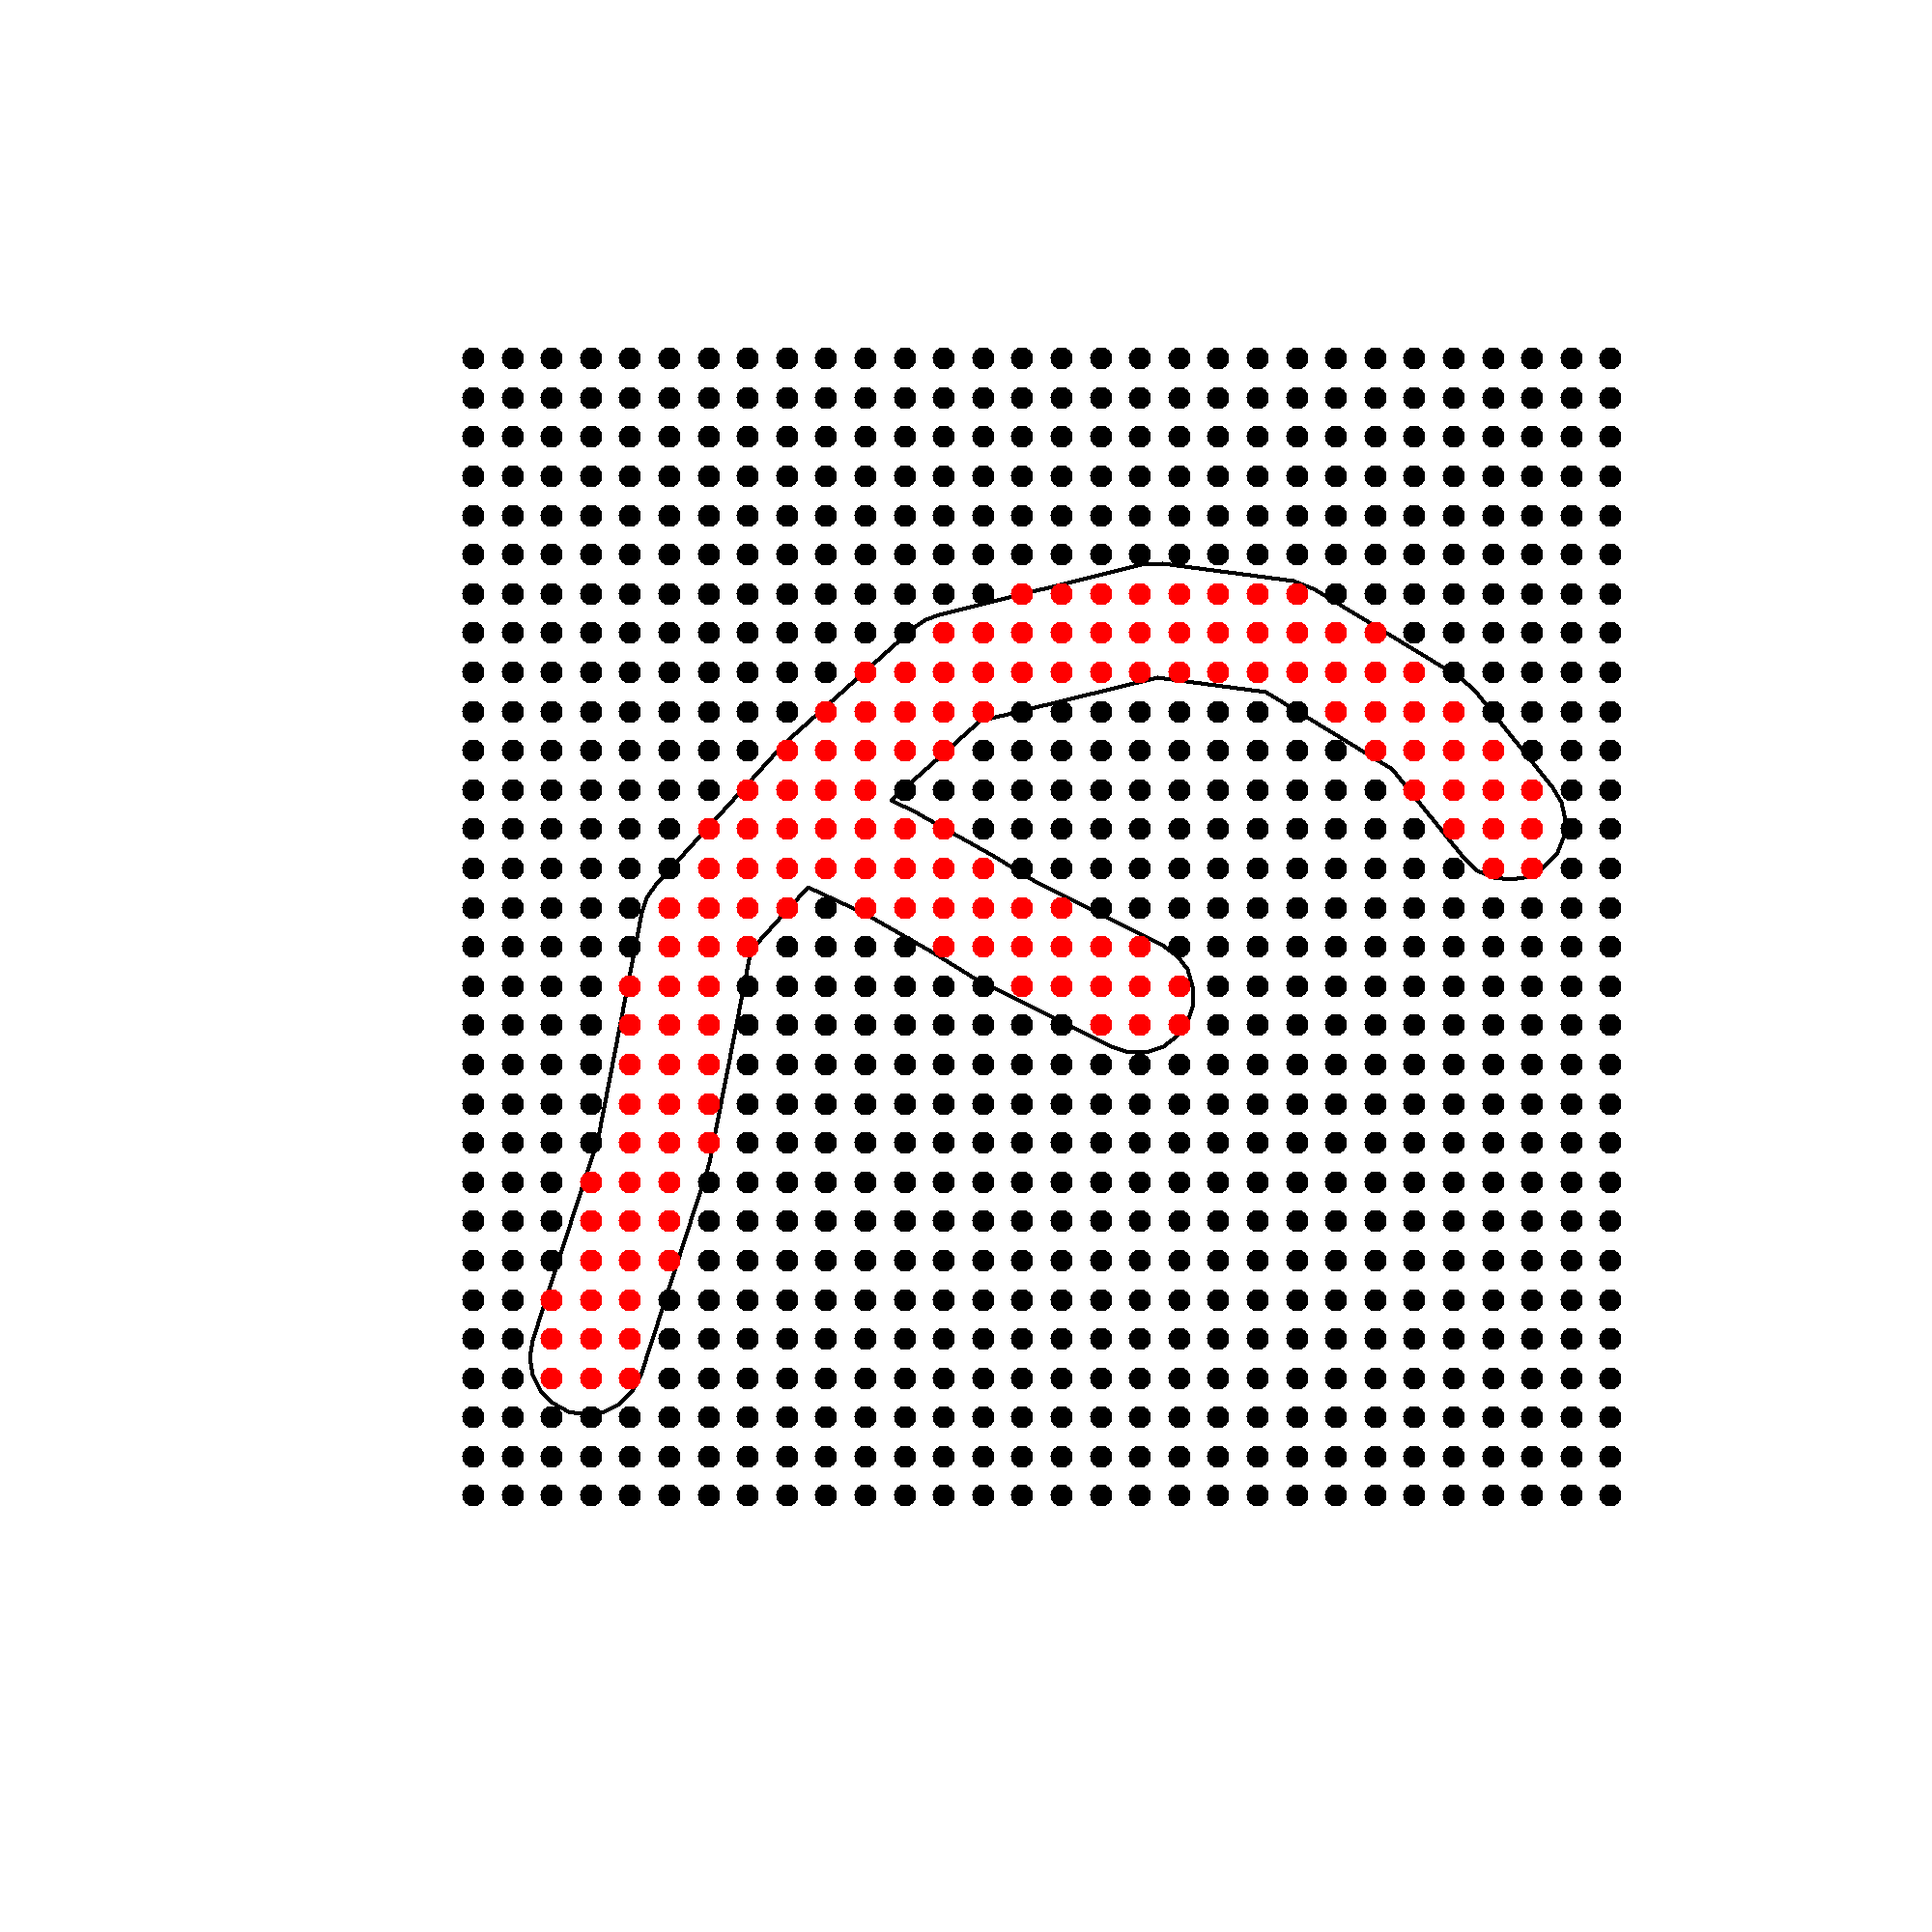
\includegraphics[height=3.25in,width=3.25in]{Ch10-EcolDist/figs/corridor}
\end{center}
\caption{A made-up wildlife corridor or reserve. The boundary outlines
  a polygon of suitable habitat surrounded by suburban development.}
\label{ecoldist.fig.corridor}
\end{figure}

In this example, we're not going to estimate parameters of the cost
function. Instead,d the point is compute ordinary Euclidean distance
but restricted by the boundaries of the corridor (or patch geometry in
general) and thus not distance ``as the crow flies.''  To do this, we
imagine that animals will tend to severely avoid leaving the buffered
habitat zone. Therefore, we assign $\mbox{\tt cost}=1$ if a pixel is
within the buffer, and $\mbox{\tt cost} = 10000$ if a pixel is outside
of a buffer. Therefore the cost to move to a neighboring pixel outside
of the buffered area is $5000.5$ compared to the cost of 1 to move to
a neighboring pixel inside the buffer.  With this cost specification,
we can compute the least-cost path distance matrix one time and modify
our likelihood code to accept the distance matrix as input. We give
that likelihood in the library \mbox{\tt scrbook} as the function
\mbox{\tt intlik3edv2}.  We note also that this function accepts a
habitat mask in the form of a vector of 0's
and 1's {\bf XXXX Kimmy: check that this is true XXXXX}
that define any potential state-space restrictions. i.e., 1 if
the pixel is an element of the state-space and 0 if it is not, and so
additional modifications to the geometry of the region could be made.
However, in the analysis of this simulated data set, we define the
state-space to be the buffered corridor system.  Here we simulate a
population of $N=200$ individuals in the corridor system and so we
restrict our state-space accordingly for purposes of fitting the
model. However we encourage you to refit the model without the
state-space restriction (for fitting the model only) and then compare
the results.  The code for doing all of this is in the help file for
\mbox{\tt intlik3edv2}, which contains the likelihood function and
sample {\bf R} script (\mbox{\tt ?intlik3edv2}).

{\small
\begin{verbatim}
### Define the cost structure
cost<-rep(NA,nrow(pts))
cost[in.pts==1]<-1      # low cost to move among pixels but not 0
cost[in.pts!=1]<-10000  # high cost

### Stuff costs into a raster
library("raster")
r<-raster(nrows=40,ncols=40)
projection(r)<- "+proj=utm +zone=12 +datum=WGS84"
extent(r)<-c(0-delta/2,10+delta/2,0-delta/2,10+delta/2)
values(r)<-matrix(cost,40,40,byrow=FALSE)

# check what it looks like
plot(r)  
points(pts,pch=20,cex=.4)

# compute ecological distances:
library("gdistance")
tr1<-transition(r,transitionFunction=function(x) 1/mean(x),directions=8)
tr1CorrC<-geoCorrection(tr1,type="c",multpl=FALSE,scl=FALSE)
costs1<-costDistance(tr1CorrC,pts)
outD<-as.matrix(costs1)
\end{verbatim}
}

In the next block of code we simulate some data and then fit a model
to the simulated data. {\bf KIMMY: I forget where ``traps'' came
  from. Is it in the ``fakecorridor'' object? Test this code XXXXXXX}
{\bf XXX ANDY: change beta to alpha1 XXXX}
{\small
\begin{verbatim}
library(``scrbook'')
traplocs<-traps$loc
trap.id<-traps$locid
ntraps<-nrow(traplocs)

set.seed(2013)
N<-200
S.possible<- (1:nrow(pts))[in.pts==1]
S.id<-sample(S.possible,N,replace=TRUE)
S<- pts[S.id,]

D<- outD[S.id,trap.id]
eD<- e2dist(S,traplocs)
Dtraps<-outD[trap.id,]

alpha0<- -1.5
sigma<- 1.5
beta<- 1/(2*sigma*sigma)
K<-10

probcap<-plogis(alpha0)*exp(-beta*D*D)
Y<-matrix(NA,nrow=N,ncol=ntraps)
for(i in 1:nrow(Y)){
 Y[i,]<-rbinom(ntraps,K,probcap[i,])
}
Y<-Y[apply(Y,1,sum)>0,]

frog1<-nlm(intlik3edv2,c(-2.5,2,log(4)),hessian=TRUE,y=Y,K=K,X=traplocs,
            S=pts,D=Dtraps,inpoly=in.pts)
frog2<-nlm(intlik3edv2,c(-2.5,2,log(4)),hessian=TRUE,y=Y,K=K,X=traplocs,
            S=pts,D=Deuclid,inpoly=in.pts)
\end{verbatim}
}

These two models fit, with the correctly specified ecological
distance, constrained by the patch boundaries, and that with the
ordinary (misspecified) Euclidean distance are summarized in Table \ref{rsf.tab.fakecorridor}.
\begin{table}
\centering
\caption{Fitting results XXXXXXXXXXXXX}
\begin{tabular}{crrrr}
Distance    &  neg. LL &    alpha0   & alpha1    &log(n0) \\ \hline
constrained & -21.8921 &  -1.3380122 & 0.3321878 & 4.3530026 \\
Euclidean   & -21.1280 &  -1.3071132 & 0.3821317 & 4.2116319 \\
\end{tabular}
\label{rsf.tab.fakecorridor}
\end{table}
We find little difference between the two models. In
particular, 150 individuals were captured and so truth is $\log(n_{0}) = 3.9$.
The correct model produces only a slightly more accurate  estimate, and
it is favored by only .7 negative log-likelihood units.
Therefore, for this single instance, the results are not too different.
This is primarily because 
 the distance between individuals, and traps that they are likely
to be captured in, is well-approximated by the Euclidean distance.




\section{Summary and Outlook}


Almost 
all published applications of SCR models to date have been based on
models for the encounter probability that are functions of the
Euclidean distance between individual activity centers and traps. The
obvious limitations of such models are that Euclidean
distance is unaffected by landscape or habitat
structure and implies stationary, isotropic and symmetrical home
ranges. These are standard criticisms of the basic SCR model which we
have seen many times in referee reports, or heard in discussions with
colleagues.
However, this should not be seen as criticism 
that is inherent to the basic conceptual formulation of SCR models, because,
we have shown here that 
one can modify the Euclidean distance metric
to accommodate more realistic 
formulations of distance that allow for inference to be made about
landscape connectivity, and model ``distance'' as a function of
local habitat characterists. As such, effective distance between individual home
range centers and traps varies depending on the local landscape. 

How animals use space and therefore how distance to a trap is
perceived by individuals is not something that can ever be known. We
can only ever conjure up models to describe this phenomenon and fit
those models to limited data on a sample of individuals during a
limited amount of time.  Here we have shown that there is hope to
estimate parameters, from capture-recapture data, that describe how
animals use space and thereby allow for irregular home range geometry
that is influenced by landscape structure.

The simulation study of \citet{royle_etal:2012ecol} demonstrated (see
Table XXXX) that the MLE of model parameters is approximately unbiased
in moderate sample sizes. Moreover, the effect of ignoring ecological
distance and using normal Euclidean distance in the model for
encounter probability, has the logical effect of causing negative bias
in estimates of $N$.  This is expected because the effect is similar
to failing to model heterogeneity, i.e., if we mis-specify ``model
$M_h$'' \citep{otis_etal:1978} with ``model $M_0$''
\citep{otis_etal:1978} then we will expect to under-estimate $N$. So
the effect of mis-specifying the ecological distance metric with a
standard homogeneous Euclidean distance has the same effect. As a
practical matter, it stands to reason that many previous applications
of SCR models based on homogeneous distance metrics have under-stated
density of the focal population.

In our view, this bias is not really the most important reason to
consider models of ecological distance. Rather, inference about the
structure of ecological distance is fundamental to many problems in
applied and theoretical ecology related to modeling landscape
connectivity, corridor and reserve design, population viability
analysis, gene flow, and other phenomena.  Models based on least-cost
path distance allow investigators to evaluate landscape factors that
influence movement of individuals over the landscape from
non-invasively collected capture-recapture data.  Therefore SCR models
based on ecological distance metrics might aid in understanding
aspects of space usage and movement in animal populations and,
ultimately, in addressing conservation-related problems such as
corridor design.

\begin{comment}
We considered inference for ecological distance models based on
marginal likelihood \citep{borchers_efford:2008}
(see Chapt. \ref{chapt.mle}).
In principle,
Bayesian analysis does not pose any unique challenges for this new
class of models, except that computing the cost-weighted distance is
computationally intensive.  So, having to do this at each iteration of
an MCMC algorithm may be impractical using existing algorithms.  A
related issue is that the size of the raster slows things down. For
very large rasters, even likelihood analysis can be computationally
challenging and methods for efficient calculation of the ecological
distance given the raster covariate(s) and parameters might be needed.
\end{comment}































\chapter{Inhomogeneous Point Process}
\label{chapt.state-space}

\chapter{Open models}
\label{chapt.open}











\bibliography{AndyRefs_alphabetized}

\end{document}